% Document collecting the table of means and mechanisms tables
\documentclass{article}
\usepackage{booktabs}
\usepackage{siunitx}
\usepackage{makecell}
\usepackage{threeparttable}
\usepackage[normalem]{ulem}
\usepackage{float}
\usepackage{amsfonts}  % Minimal
\usepackage{amssymb}   % Includes amsfonts and more
\usepackage{amsmath}
% Additional packages for landscape pages
\usepackage{dsfont}
\usepackage{pdflscape}
\usepackage{tabularx}

\usepackage{tabularx,array}
\usepackage{graphicx}
% define a “centering” version of X
\newcolumntype{C}{>{\centering\arraybackslash}X}

%\setlength{\tabcolsep}{8pt}

% Base directory for cleaned results
\newcommand{\cleanedresultsdir}{../results/cleaned}
% Base directory for figures
\newcommand{\figdir}{../results/figures}

\begin{document}

% -------------------------------------------------------------------------
%  Figures – key descriptive plots
% -------------------------------------------------------------------------
\section{Figures}

\begin{figure}[H]
  \centering
  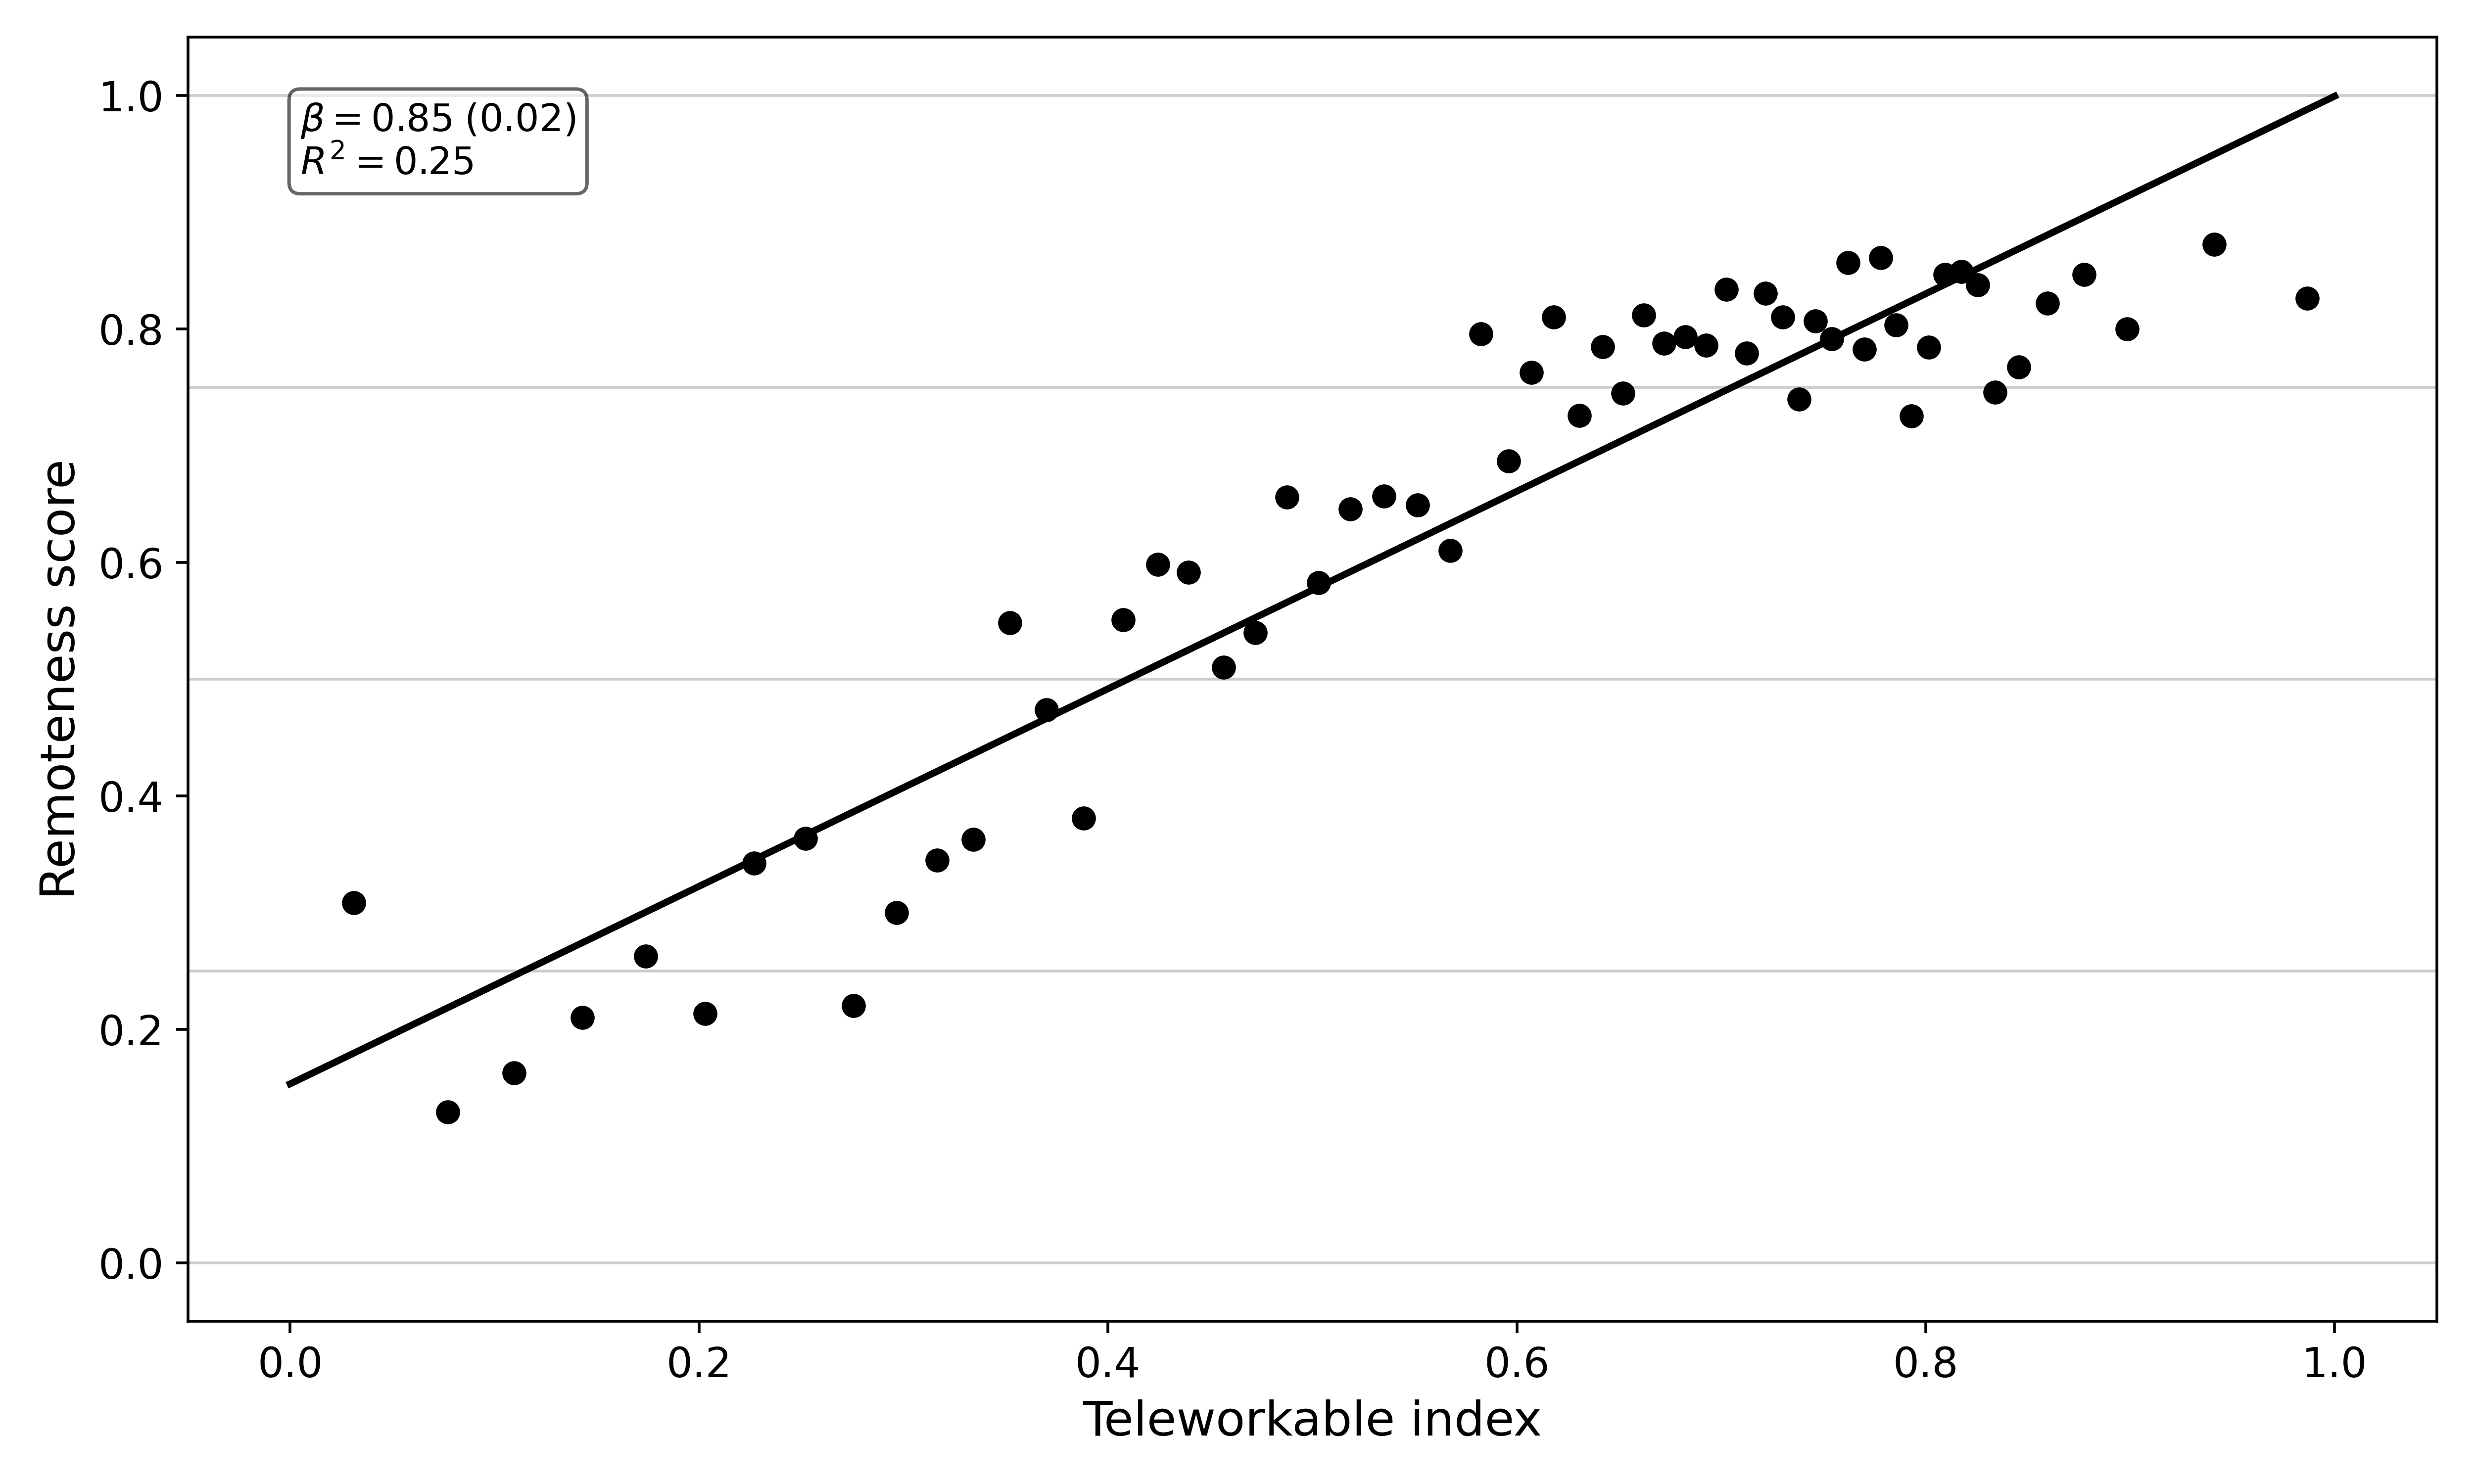
\includegraphics[width=0.9\textwidth]{\figdir/firm_teleworkable_remote.png}
  \caption{Remote v. Teleworkabe Scores}
\end{figure}

\begin{figure}[H]
  \centering
  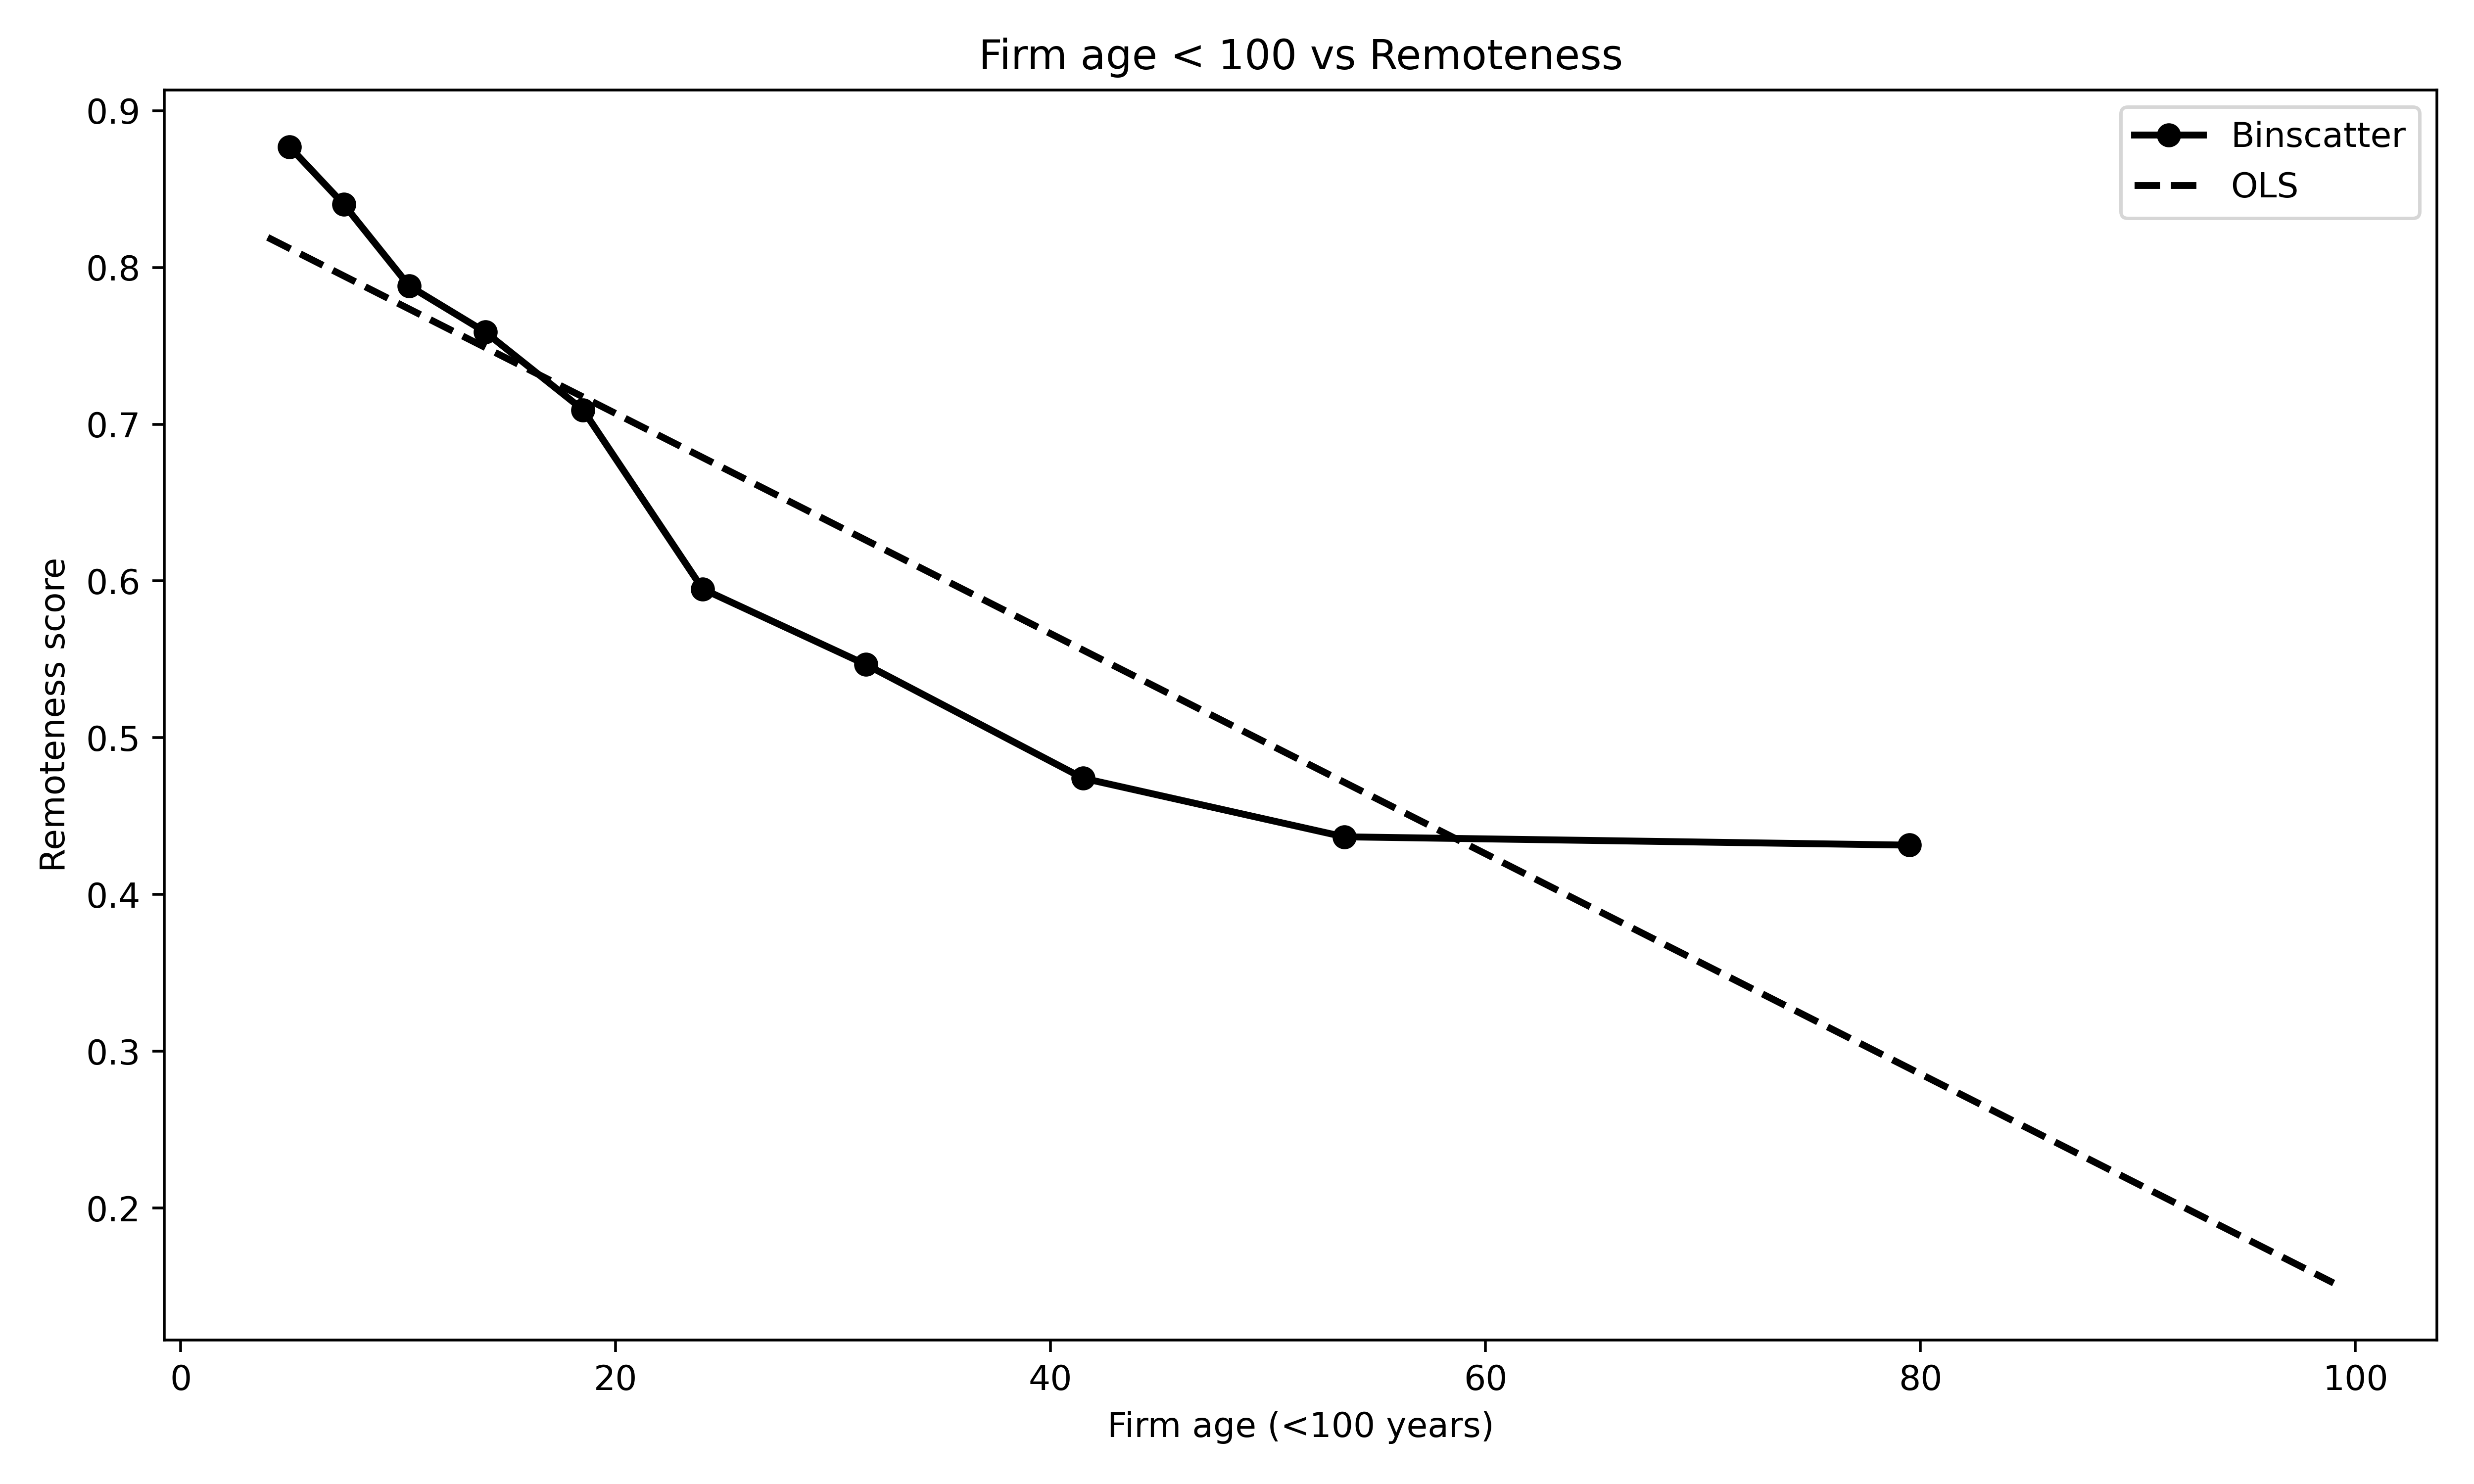
\includegraphics[width=0.9\textwidth]{\figdir/firm_age_lt100_remote.png}
  \caption{Remote v. Firm Age}
\end{figure}

%\clearpage

\section{Table of Means}
\begin{table}[H]
        \centering
        \begin{threeparttable}
        \caption{Table of Means}
        \label{tab:means}
        \begin{tabular}{lcc@{\hspace{6pt}}c}
        \toprule
         & Startup & Incumbent & All Firms \\
        \midrule
        \addlinespace
        \multicolumn{4}{l}{\textbf{\uline{Panel A: Firm-level}}}\\[0.3em]
        Growth & \makecell{0.20 \\ (0.31)} & \makecell{0.06 \\ (0.16)} & \makecell{0.09 \\ (0.22)} \\
Leave & \makecell{0.26 \\ (0.31)} & \makecell{0.21 \\ (0.28)} & \makecell{0.22 \\ (0.29)} \\
Join & \makecell{0.35 \\ (0.32)} & \makecell{0.17 \\ (0.18)} & \makecell{0.22 \\ (0.24)} \\
Teleworkable Score \,(0--1) & \makecell{0.67 \\ (0.18)} & \makecell{0.54 \\ (0.25)} & \makecell{0.57 \\ (0.24)} \\
Remote Score \,(0--1) & \makecell{0.85 \\ (0.30)} & \makecell{0.57 \\ (0.41)} & \makecell{0.64 \\ (0.40)} \\
Employees (Count) & \makecell{271 \\ (1432)} & \makecell{2740 \\ (9555)} & \makecell{2126 \\ (8380)} \\
Age & \makecell{7 \\ (2)} & \makecell{43 \\ (34)} & \makecell{34 \\ (33)} \\
Rent (\textdollar/sq ft) & \makecell{49 \\ (21)} & \makecell{37 \\ (19)} & \makecell{40 \\ (20)} \\
Centrality Score & \makecell{1419 \\ (1830)} & \makecell{949 \\ (1309)} & \makecell{1066 \\ (1470)} \\
Seniority Levels (Count) & \makecell{3.62 \\ (0.77)} & \makecell{3.86 \\ (0.50)} & \makecell{3.80 \\ (0.59)} \\
\addlinespace
\midrule
Number of firms & 878 & 2630 & 3508 \\
Observations & 10450 & 31530 & 41980 \\
        \addlinespace
        \midrule
        \addlinespace
        \multicolumn{4}{l}{\textbf{\uline{Panel B: User-level}}}\\[0.3em]
        Total Contributions & \makecell{363.55 \\ (796.33)} & \makecell{193.43 \\ (641.42)} & \makecell{225.69 \\ (676.83)} \\
Restricted Contributions & \makecell{319.21 \\ (727.47)} & \makecell{138.68 \\ (356.21)} & \makecell{172.91 \\ (456.26)} \\
\addlinespace
\midrule
Number of firms & 727 & 1530 & 2257 \\
Number of users & 8635 & 33351 & 38411 \\
Observations & 48756 & 208390 & 257146 \\
        \bottomrule
        \end{tabular}
        \begin{tablenotes}[flushleft]
\footnotesize
\item \emph{Notes}: Panel~A uses firm--half--year observations. Panel~B relies on worker--half--year observations. ``Number of firms'' counts distinct firm\,IDs that ever appear in each category over the full sample window, so Startup and Incumbent counts need not sum to the ``All'' column. \textit{Growth}, \textit{Leave}, and \textit{Join} rates are fractions between 0 and 1. \textit{Teleworkable} and \textit{Remote} scores are index values between~0 and~1.  The sample period spans 2016 H2–2022 H1 at the firm level and 2017 H1–2022 H1 at the user level.
\end{tablenotes}
        \end{threeparttable}
        \end{table}


%-----------------------------------------------------------------
%=====================================================================
% Firm Scaling
%=====================================================================

\clearpage
\section{Firm Scaling}
\label{sec:firm_scaling}

\subsection{OLS}
% ------------------------------------------------------------------
%  Firm-Scaling: Two-panel OLS results
% ------------------------------------------------------------------

\begin{table}[H]
\centering
\caption{Firm Scaling OLS}
\label{tab:firm_scaling_ols}
\centering

    \begin{tabular*}{\textwidth}{@{}l@{\extracolsep{\fill}}cccc@{}}
    \toprule
    \multicolumn{5}{@{}l}{\textbf{\uline{Panel A: FE Variants}}}\\
\addlinespace
     & \multicolumn{4}{c}{Growth} \\
    \cmidrule(lr){2-5}
     & (1) & (2) & (3) & (4) \\
    \midrule
    $ \text{Remote} \times \mathds{1}(\text{Post}) $ & \makecell[c]{0.00\\(0.00)} & \makecell[c]{0.00\\(0.00)} & \makecell[c]{0.00\\(0.00)} & \makecell[c]{0.00\\(0.00)} \\
$ \text{Remote} \times \mathds{1}(\text{Post}) \times \text{Startup} $ & \makecell[c]{0.07***\\(0.02)} & \makecell[c]{0.07***\\(0.02)} & \makecell[c]{0.07***\\(0.02)} & \makecell[c]{0.07***\\(0.02)} \\
    \midrule
    Time FE &  &  & $\checkmark$ & $\checkmark$ \\
Firm FE &  & $\checkmark$ &  & $\checkmark$ \\
    \midrule
    N & 41,980 & 41,980 & 41,980 & 41,980 \\
    \specialrule{\lightrulewidth}{0pt}{0pt}
    \end{tabular*}
\vspace{0.75em}
\begin{tabular*}{\textwidth}{@{}l@{\extracolsep{\fill}}ccc@{}}

    \multicolumn{4}{@{}l}{\textbf{\uline{Panel B: Base Specification}}}\\
\addlinespace
     & \multicolumn{3}{c}{Outcome} \\
    \cmidrule(lr){2-4}
     & Growth & Join & Leave \\
    \midrule
    $ \text{Remote} \times \mathds{1}(\text{Post}) $ & \makecell[c]{0.00\\(0.00)} & \makecell[c]{0.01**\\(0.00)} & \makecell[c]{0.02***\\(0.00)} \\
$ \text{Remote} \times \mathds{1}(\text{Post}) \times \text{Startup} $ & \makecell[c]{0.07***\\(0.02)} & \makecell[c]{0.05*\\(0.03)} & \makecell[c]{-0.01\\(0.01)} \\
    \midrule
    N & 41,980 & 41,980 & 41,980 \\
    \bottomrule
    \end{tabular*}
\end{table}


\subsection{Instrumental Variables}
\begin{table}[H]
\centering
{\scriptsize\centering
  \caption{Firm Scaling — IV}
  \label{tab:firm_scaling_iv}
}
\centering
{\scriptsize%
\setlength{\tabcolsep}{3pt}%
\renewcommand{\arraystretch}{0.95}%
\begin{adjustbox}{max width=\linewidth, max height=0.9\textheight, center}%

    \begin{tabularx}{\linewidth}{l@{\hspace{4pt}}>{\centering\arraybackslash}X@{\hspace{4pt}}@{\hspace{4pt}}>{\centering\arraybackslash}X@{\hspace{4pt}}@{\hspace{4pt}}>{\centering\arraybackslash}X@{\hspace{4pt}}@{\hspace{4pt}}>{\centering\arraybackslash}X@{\hspace{4pt}}}
    \toprule
     & (1) & (2) & (3) & (4) \\
    \midrule
     & \makecell[c]{Growth\\(wins.)} & \makecell[c]{Growth\\(wins.)} & \makecell[c]{Join\\(wins.)} & \makecell[c]{Leave\\(wins.)} \\
    \midrule
    $ \text{Remote} \times \mathds{1}(\text{Post}) $ & \makecell[c]{0.02\\(0.01)} & \makecell[c]{-0.00\\(0.01)} & \makecell[c]{0.03***\\(0.01)} & \makecell[c]{0.04***\\(0.00)} \\
$ \text{Remote} \times \mathds{1}(\text{Post}) \times \text{Startup} $ &  & \makecell[c]{0.22**\\(0.09)} & \makecell[c]{0.23**\\(0.10)} & \makecell[c]{0.06\\(0.05)} \\
    \midrule
    Time FE & $\checkmark$ & $\checkmark$ & $\checkmark$ & $\checkmark$ \\
Firm FE & $\checkmark$ & $\checkmark$ & $\checkmark$ & $\checkmark$ \\
    \midrule
    Pre-COVID mean & 0.11 & 0.11 & 0.25 & 0.14 \\
    N & 41,742 & 41,742 & 41,742 & 41,742 \\
    KP rk Wald F & 982.73 & 18.30 & 18.30 & 18.30 \\
    \bottomrule
    \end{tabularx}\end{adjustbox}}
\end{table}


\subsection{First Stage}
% Auto-generated first-stage estimates – Firm Scaling
\begin{table}[H]
\centering
\caption{First-Stage Estimates – Firm Scaling}
\label{tab:firm_scaling_first_stage}
\begin{tabular}{lcc}
\toprule
 & $ \text{Remote} \times \mathds{1}(\text{Post}) $ & $ \text{Remote} \times \mathds{1}(\text{Post}) \times \text{Startup} $\\
\midrule
$ \text{Teleworkable} \times \mathds{1}(\text{Post}) $ & \makecell[c]{0.826***\\(0.028)} & \makecell[c]{-0.000\\(0.000)}\\
$ \text{Teleworkable} \times \mathds{1}(\text{Post}) \times \text{Startup} $ & \makecell[c]{-0.412***\\(0.077)} & \makecell[c]{0.414***\\(0.072)}\\
$ \mathds{1}(\text{Post}) \times \text{Startup} $ & \makecell[c]{0.455***\\(0.055)} & \makecell[c]{0.575***\\(0.052)}\\
\midrule
Time FE & $\checkmark$ & $\checkmark$\\
Firm FE & $\checkmark$ & $\checkmark$\\
\midrule
Partial F & 437.86 & 16.54\\
N & 41,980 & 41,980\\
\bottomrule
\end{tabular}
\end{table}


% ------------------------------------------------------------------
%  Remote vs. Teleworkable – Basic First Stage
% ------------------------------------------------------------------
\subsection{Remote $\rightarrow$ Teleworkable: First Stage}
% Auto-generated – Remote on Teleworkable first stage
\begin{table}[H]
\centering
\caption{First-Stage Estimate: Remote $\rightarrow$ Teleworkable}
\label{tab:remote_first_stage}
\begin{tabular}{lc}
\toprule
 & $ \text{Remote} $\\
\midrule
$ \text{Teleworkable} $ & \makecell[c]{0.795***\\(0.021)}\\
\midrule
$R^2$ & 0.290\\
N & 3,486\\
\bottomrule
\end{tabular}
\end{table}


%-----------------------------------------------------------------
%=====================================================================
% User Productivity
%=====================================================================

\clearpage
\section{User Productivity}
\label{sec:user_productivity}

\subsection{OLS -- Unbalanced Panel}
% Auto-generated user productivity table

\begin{table}[H]
\centering
\caption{User Productivity (unbalanced) -- OLS}
\label{tab:user_productivity_unbalanced_ols}
\centering

    \begin{tabularx}{\dimexpr\textwidth + 2cm\relax}{@{}l@{\hskip 8pt}>{\centering\arraybackslash}X@{\hskip 8pt}>{\centering\arraybackslash}X@{\hskip 8pt}>{\centering\arraybackslash}X@{\hskip 8pt}>{\centering\arraybackslash}X@{\hskip 8pt}>{\centering\arraybackslash}X@{\hskip 8pt}>{\centering\arraybackslash}X@{}}
    \toprule
    \multicolumn{7}{@{}l}{\textbf{\uline{Panel A: Total Contrib. (pct. rk)}}}\\
\addlinespace


     & (1) & (2) & (3) & (4) & (5) & (6) \\
    \midrule
    $ \text{Remote} \times \mathds{1}(\text{Post}) $ & \makecell[c]{0.29\\(0.24)} & \makecell[c]{0.32\\(0.25)} & \makecell[c]{0.27\\(0.26)} & \makecell[c]{0.16\\(0.26)} & \makecell[c]{0.34\\(0.26)} & \makecell[c]{0.29\\(0.29)} \\
$ \text{Remote} \times \mathds{1}(\text{Post}) \times \text{Startup} $ &  & \makecell[c]{-0.40\\(0.81)} & \makecell[c]{0.19\\(0.84)} & \makecell[c]{-0.49\\(0.83)} & \makecell[c]{-0.42\\(0.82)} & \makecell[c]{-0.83\\(0.88)} \\
    \midrule
    Time FE & $\checkmark$ & $\checkmark$ & $\checkmark$ &  &  &  \\
Firm FE & $\checkmark$ & $\checkmark$ &  & $\checkmark$ & $\checkmark$ & $\checkmark$ \\
User FE & $\checkmark$ & $\checkmark$ &  & $\checkmark$ & $\checkmark$ & $\checkmark$ \\
Firm $\times$ User FE &  &  & $\checkmark$ &  &  &  \\
Industry $\times$ Time FE &  &  &  & $\checkmark$ &  & $\checkmark$ \\
MSA $\times$ Time FE &  &  &  &  & $\checkmark$ & $\checkmark$ \\
    \midrule
    N & 1,226,001 & 1,226,001 & 1,209,078 & 1,218,407 & 1,225,589 & 1,208,970 \\
    \specialrule{\lightrulewidth}{0pt}{0pt}
    \end{tabularx}

    \begin{tabularx}{\dimexpr\textwidth + 2cm\relax}{@{}l@{\hskip 8pt}>{\centering\arraybackslash}X@{\hskip 8pt}>{\centering\arraybackslash}X@{\hskip 8pt}>{\centering\arraybackslash}X@{}}

    \multicolumn{4}{@{}l}{\textbf{\uline{Panel B: Additional Outcomes}}}\\
\addlinespace
     & \multicolumn{3}{c}{Outcome} \\
    \cmidrule(lr){2-4}
     & Restricted (pct. rk) & Total (wins.) & Restr. (wins.) \\
    \midrule
    $ \text{Remote} \times \mathds{1}(\text{Post}) $ & \makecell[c]{-0.28**\\(0.12)} & \makecell[c]{-0.51\\(0.52)} & \makecell[c]{-0.20\\(0.29)} \\
$ \text{Remote} \times \mathds{1}(\text{Post}) \times \text{Startup} $ & \makecell[c]{1.93***\\(0.49)} & \makecell[c]{5.22**\\(2.47)} & \makecell[c]{5.37***\\(1.56)} \\
    \midrule
    Pre-COVID mean & 16.32 & 34.87 & 15.82 \\
    N & 1,226,001 & 1,226,001 & 1,226,001 \\

    \bottomrule
    \end{tabularx}
\end{table}


\subsection{OLS -- Balanced Panel}
% Auto-generated user productivity table

\begin{table}[H]
\centering
\caption{User Productivity (balanced) -- OLS}
\label{tab:user_productivity_balanced_ols}
\centering

    \begin{tabularx}{\dimexpr\textwidth + 2cm\relax}{@{}l@{\hskip 8pt}>{\centering\arraybackslash}X@{\hskip 8pt}>{\centering\arraybackslash}X@{\hskip 8pt}>{\centering\arraybackslash}X@{\hskip 8pt}>{\centering\arraybackslash}X@{\hskip 8pt}>{\centering\arraybackslash}X@{\hskip 8pt}>{\centering\arraybackslash}X@{}}
    \toprule
    \multicolumn{7}{@{}l}{\textbf{\uline{Panel A: Total Contrib. (pct. rk)}}}\\
\addlinespace


     & (1) & (2) & (3) & (4) & (5) & (6) \\
    \midrule
    $ \text{Remote} \times \mathds{1}(\text{Post}) $ & \makecell[c]{0.31\\(0.38)} & \makecell[c]{0.48\\(0.39)} & \makecell[c]{0.51\\(0.40)} & \makecell[c]{0.43\\(0.40)} & \makecell[c]{0.41\\(0.41)} & \makecell[c]{0.11\\(0.46)} \\
$ \text{Remote} \times \mathds{1}(\text{Post}) \times \text{Startup} $ &  & \makecell[c]{-3.48**\\(1.55)} & \makecell[c]{-3.64**\\(1.60)} & \makecell[c]{-3.76**\\(1.60)} & \makecell[c]{-3.39**\\(1.57)} & \makecell[c]{-3.40**\\(1.69)} \\
    \midrule
    Time FE & $\checkmark$ & $\checkmark$ & $\checkmark$ &  &  &  \\
Firm FE & $\checkmark$ & $\checkmark$ &  & $\checkmark$ & $\checkmark$ & $\checkmark$ \\
User FE & $\checkmark$ & $\checkmark$ &  & $\checkmark$ & $\checkmark$ & $\checkmark$ \\
Firm $\times$ User FE &  &  & $\checkmark$ &  &  &  \\
Industry $\times$ Time FE &  &  &  & $\checkmark$ &  & $\checkmark$ \\
MSA $\times$ Time FE &  &  &  &  & $\checkmark$ & $\checkmark$ \\
    \midrule
    N & 519,099 & 519,099 & 516,442 & 515,817 & 518,431 & 508,510 \\
    \specialrule{\lightrulewidth}{0pt}{0pt}
    \end{tabularx}

    \begin{tabularx}{\dimexpr\textwidth + 2cm\relax}{@{}l@{\hskip 8pt}>{\centering\arraybackslash}X@{\hskip 8pt}>{\centering\arraybackslash}X@{\hskip 8pt}>{\centering\arraybackslash}X@{}}

    \multicolumn{4}{@{}l}{\textbf{\uline{Panel B: Additional Outcomes}}}\\
\addlinespace
     & \multicolumn{3}{c}{Outcome} \\
    \cmidrule(lr){2-4}
     & Restricted (pct. rk) & Total (wins.) & Restr. (wins.) \\
    \midrule
    $ \text{Remote} \times \mathds{1}(\text{Post}) $ & \makecell[c]{-0.07\\(0.11)} & \makecell[c]{-0.61\\(0.59)} & \makecell[c]{-0.05\\(0.19)} \\
$ \text{Remote} \times \mathds{1}(\text{Post}) \times \text{Startup} $ & \makecell[c]{1.00\\(0.62)} & \makecell[c]{0.60\\(3.27)} & \makecell[c]{1.08\\(1.14)} \\
    \midrule
    Pre-COVID mean & 9.70 & 26.48 & 7.04 \\
    N & 519,099 & 519,099 & 519,099 \\

    \bottomrule
    \end{tabularx}
\end{table}


\subsection{OLS -- Pre-COVID Panel}
\begin{table}[H]
\centering
{\scriptsize\centering
  \caption{User Productivity -- OLS}
  \label{tab:user_productivity_precovid_ols}
}
\centering
{\scriptsize%
\setlength{\tabcolsep}{3pt}%
\renewcommand{\arraystretch}{0.95}%
\begin{adjustbox}{max width=\linewidth, max height=0.9\textheight, center}%

\begin{tabularx}{\linewidth}{l@{\hspace{4pt}}>{\centering\arraybackslash}X@{\hspace{4pt}}@{\hspace{4pt}}>{\centering\arraybackslash}X@{\hspace{4pt}}@{\hspace{4pt}}>{\centering\arraybackslash}X@{\hspace{4pt}}@{\hspace{4pt}}>{\centering\arraybackslash}X@{\hspace{4pt}}@{\hspace{4pt}}>{\centering\arraybackslash}X@{\hspace{4pt}}@{\hspace{4pt}}>{\centering\arraybackslash}X@{\hspace{4pt}}}
\toprule
 & (1) & (2) & (3) & (4) & (5) & (6) \\
\midrule
 & \makecell[c]{Total\\(pct.\ rk.)} & \makecell[c]{Total\\(pct.\ rk.)} & \makecell[c]{Total\\(pct.\ rk.)} & \makecell[c]{Restr.\\(pct.\ rk.)} & \makecell[c]{Total\\(wins.)} & \makecell[c]{Restr.\\(wins.)} \\
\midrule
$ \text{Remote} \times \mathds{1}(\text{Post}) $ & \makecell[c]{-0.28\\(0.44)} & \makecell[c]{-1.03**\\(0.48)} & \makecell[c]{-1.23**\\(0.50)} & \makecell[c]{-1.48***\\(0.52)} & \makecell[c]{-19.74***\\(4.66)} & \makecell[c]{-17.33***\\(3.91)} \\
$ \text{Remote} \times \mathds{1}(\text{Post}) \times \text{Startup} $ &  & \makecell[c]{5.18***\\(1.24)} & \makecell[c]{6.21***\\(1.27)} & \makecell[c]{7.31***\\(1.27)} & \makecell[c]{59.23***\\(14.22)} & \makecell[c]{55.41***\\(12.74)} \\
\midrule
Time FE & $\checkmark$ & $\checkmark$ & $\checkmark$ & $\checkmark$ & $\checkmark$ & $\checkmark$ \\
Firm FE & $\checkmark$ & $\checkmark$ &  &  &  &  \\
User FE & $\checkmark$ & $\checkmark$ &  &  &  &  \\
Firm $\times$ User FE &  &  & $\checkmark$ & $\checkmark$ & $\checkmark$ & $\checkmark$ \\
\midrule
    Pre-COVID mean & 49.92 & 49.92 & 49.92 & 48.48 & 184.71 & 138.15 \\

    N & 229,862 & 229,862 & 224,708 & 224,708 & 224,708 & 224,708 \\
\bottomrule
\end{tabularx}\end{adjustbox}}
\end{table}


\subsection{Instrumental Variables -- Unbalanced Panel}
% Auto-generated user productivity table

\begin{table}[H]
\centering
\caption{User Productivity (unbalanced) -- IV}
\label{tab:user_productivity_unbalanced_iv}
\centering

    \begin{tabularx}{\dimexpr\textwidth + 2cm\relax}{@{}l@{\hskip 8pt}>{\centering\arraybackslash}X@{\hskip 8pt}>{\centering\arraybackslash}X@{\hskip 8pt}>{\centering\arraybackslash}X@{\hskip 8pt}>{\centering\arraybackslash}X@{\hskip 8pt}>{\centering\arraybackslash}X@{\hskip 8pt}>{\centering\arraybackslash}X@{}}
    \toprule
    \multicolumn{7}{@{}l}{\textbf{\uline{Panel A: Total Contrib. (pct. rk)}}}\\
\addlinespace


     & (1) & (2) & (3) & (4) & (5) & (6) \\
    \midrule
    $ \text{Remote} \times \mathds{1}(\text{Post}) $ & \makecell[c]{15.34***\\(2.31)} & \makecell[c]{18.02***\\(2.77)} & \makecell[c]{15.22***\\(2.86)} & \makecell[c]{24.35***\\(6.59)} & \makecell[c]{15.79***\\(2.42)} & \makecell[c]{11.26\\(7.86)} \\
$ \text{Remote} \times \mathds{1}(\text{Post}) \times \text{Startup} $ &  & \makecell[c]{-14.02***\\(4.20)} & \makecell[c]{-12.53***\\(4.25)} & \makecell[c]{-16.61***\\(4.88)} & \makecell[c]{-12.82***\\(4.07)} & \makecell[c]{-9.02*\\(5.01)} \\
    \midrule
    Time FE & $\checkmark$ & $\checkmark$ & $\checkmark$ &  &  &  \\
Firm FE & $\checkmark$ & $\checkmark$ &  & $\checkmark$ & $\checkmark$ & $\checkmark$ \\
User FE & $\checkmark$ & $\checkmark$ &  & $\checkmark$ & $\checkmark$ & $\checkmark$ \\
Firm $\times$ User FE &  &  & $\checkmark$ &  &  &  \\
Industry $\times$ Time FE &  &  &  & $\checkmark$ &  & $\checkmark$ \\
MSA $\times$ Time FE &  &  &  &  & $\checkmark$ & $\checkmark$ \\
    \midrule
    N & 1,226,437 & 1,226,437 & 1,209,494 & 1,218,839 & 1,226,025 & 1,209,405 \\
KP rk Wald F & 1090.65 & 382.38 & 329.92 & 103.64 & 536.93 & 79.14 \\
    \specialrule{\lightrulewidth}{0pt}{0pt}
    \end{tabularx}

    \begin{tabularx}{\dimexpr\textwidth + 2cm\relax}{@{}l@{\hskip 8pt}>{\centering\arraybackslash}X@{\hskip 8pt}>{\centering\arraybackslash}X@{\hskip 8pt}>{\centering\arraybackslash}X@{}}

    \multicolumn{4}{@{}l}{\textbf{\uline{Panel B: Additional Outcomes}}}\\
\addlinespace
     & \multicolumn{3}{c}{Outcome} \\
    \cmidrule(lr){2-4}
     & Restricted (pct. rk) & Total (wins.) & Restr. (wins.) \\
    \midrule
    $ \text{Remote} \times \mathds{1}(\text{Post}) $ & \makecell[c]{0.24\\(1.19)} & \makecell[c]{-1.28\\(4.70)} & \makecell[c]{-5.45**\\(2.62)} \\
$ \text{Remote} \times \mathds{1}(\text{Post}) \times \text{Startup} $ & \makecell[c]{1.76\\(2.18)} & \makecell[c]{2.59\\(11.81)} & \makecell[c]{11.38\\(7.31)} \\
    \midrule
    Pre-COVID mean & 16.33 & 34.89 & 15.84 \\
    N & 1,226,437 & 1,226,437 & 1,226,437 \\
    KP rk Wald F & 382.38 & 382.38 & 382.38 \\
    \bottomrule
    \end{tabularx}
\end{table}


\subsection{Instrumental Variables -- Balanced Panel}
% Auto-generated user productivity table

\begin{table}[H]
\centering
\caption{User Productivity (balanced) -- IV}
\label{tab:user_productivity_balanced_iv}
\centering

    \begin{tabularx}{\dimexpr\textwidth + 2cm\relax}{@{}l@{\hskip 8pt}>{\centering\arraybackslash}X@{\hskip 8pt}>{\centering\arraybackslash}X@{\hskip 8pt}>{\centering\arraybackslash}X@{\hskip 8pt}>{\centering\arraybackslash}X@{\hskip 8pt}>{\centering\arraybackslash}X@{\hskip 8pt}>{\centering\arraybackslash}X@{}}
    \toprule
    \multicolumn{7}{@{}l}{\textbf{\uline{Panel A: Total Contrib. (pct. rk)}}}\\
\addlinespace


     & (1) & (2) & (3) & (4) & (5) & (6) \\
    \midrule
    $ \text{Remote} \times \mathds{1}(\text{Post}) $ & \makecell[c]{17.80***\\(3.96)} & \makecell[c]{19.24***\\(4.46)} & \makecell[c]{17.37***\\(4.48)} & \makecell[c]{19.07\\(18.16)} & \makecell[c]{16.64***\\(3.72)} & \makecell[c]{-4.54\\(23.63)} \\
$ \text{Remote} \times \mathds{1}(\text{Post}) \times \text{Startup} $ &  & \makecell[c]{-10.96\\(8.12)} & \makecell[c]{-13.31\\(8.23)} & \makecell[c]{-12.50\\(10.56)} & \makecell[c]{-9.70\\(7.92)} & \makecell[c]{-0.90\\(9.15)} \\
    \midrule
    Time FE & $\checkmark$ & $\checkmark$ & $\checkmark$ &  &  &  \\
Firm FE & $\checkmark$ & $\checkmark$ &  & $\checkmark$ & $\checkmark$ & $\checkmark$ \\
User FE & $\checkmark$ & $\checkmark$ &  & $\checkmark$ & $\checkmark$ & $\checkmark$ \\
Firm $\times$ User FE &  &  & $\checkmark$ &  &  &  \\
Industry $\times$ Time FE &  &  &  & $\checkmark$ &  & $\checkmark$ \\
MSA $\times$ Time FE &  &  &  &  & $\checkmark$ & $\checkmark$ \\
    \midrule
    N & 519,099 & 519,099 & 516,442 & 515,817 & 518,431 & 508,510 \\
KP rk Wald F & 323.34 & 128.03 & 120.82 & 11.52 & 195.26 & 7.50 \\
    \specialrule{\lightrulewidth}{0pt}{0pt}
    \end{tabularx}

    \begin{tabularx}{\dimexpr\textwidth + 2cm\relax}{@{}l@{\hskip 8pt}>{\centering\arraybackslash}X@{\hskip 8pt}>{\centering\arraybackslash}X@{\hskip 8pt}>{\centering\arraybackslash}X@{}}

    \multicolumn{4}{@{}l}{\textbf{\uline{Panel B: Additional Outcomes}}}\\
\addlinespace
     & \multicolumn{3}{c}{Outcome} \\
    \cmidrule(lr){2-4}
     & Restricted (pct. rk) & Total (wins.) & Restr. (wins.) \\
    \midrule
    $ \text{Remote} \times \mathds{1}(\text{Post}) $ & \makecell[c]{-0.35\\(1.23)} & \makecell[c]{-8.04\\(6.99)} & \makecell[c]{-6.13*\\(3.60)} \\
$ \text{Remote} \times \mathds{1}(\text{Post}) \times \text{Startup} $ & \makecell[c]{6.04*\\(3.44)} & \makecell[c]{40.55*\\(23.35)} & \makecell[c]{37.12***\\(14.11)} \\
    \midrule
    Pre-COVID mean & 9.52 & 29.47 & 11.86 \\
    N & 519,099 & 519,099 & 519,099 \\
    KP rk Wald F & 128.03 & 128.03 & 128.03 \\
    \bottomrule
    \end{tabularx}
\end{table}


\subsection{Instrumental Variables -- Pre-COVID Panel}
% Auto-generated user productivity table

\begin{table}[H]
\centering
\caption{User Productivity (precovid) -- IV}
\label{tab:user_productivity_precovid_iv}
\centering

    \begin{tabularx}{\dimexpr\textwidth + 2cm\relax}{@{}l@{\hskip 8pt}>{\centering\arraybackslash}X@{\hskip 8pt}>{\centering\arraybackslash}X@{\hskip 8pt}>{\centering\arraybackslash}X@{\hskip 8pt}>{\centering\arraybackslash}X@{\hskip 8pt}>{\centering\arraybackslash}X@{\hskip 8pt}>{\centering\arraybackslash}X@{}}
    \toprule
    \multicolumn{7}{@{}l}{\textbf{\uline{Panel A: Total Contrib. (pct. rk)}}}\\
\addlinespace


     & (1) & (2) & (3) & (4) & (5) & (6) \\
    \midrule
    $ \text{Remote} \times \mathds{1}(\text{Post}) $ & \makecell[c]{4.10\\(2.74)} & \makecell[c]{3.88\\(4.00)} & \makecell[c]{2.24\\(4.04)} & \makecell[c]{10.69**\\(5.44)} & \makecell[c]{3.83\\(4.30)} & \makecell[c]{8.99\\(8.33)} \\
$ \text{Remote} \times \mathds{1}(\text{Post}) \times \text{Startup} $ &  & \makecell[c]{0.61\\(4.86)} & \makecell[c]{1.16\\(4.78)} & \makecell[c]{-3.35\\(4.68)} & \makecell[c]{0.39\\(5.41)} & \makecell[c]{-4.77\\(6.46)} \\
    \midrule
    Time FE & $\checkmark$ & $\checkmark$ & $\checkmark$ &  &  &  \\
Firm FE & $\checkmark$ & $\checkmark$ &  & $\checkmark$ & $\checkmark$ & $\checkmark$ \\
User FE & $\checkmark$ & $\checkmark$ &  & $\checkmark$ & $\checkmark$ & $\checkmark$ \\
Firm $\times$ User FE &  &  & $\checkmark$ &  &  &  \\
Industry $\times$ Time FE &  &  &  & $\checkmark$ &  & $\checkmark$ \\
MSA $\times$ Time FE &  &  &  &  & $\checkmark$ & $\checkmark$ \\
    \midrule
    N & 229,862 & 229,862 & 224,708 & 227,829 & 229,043 & 222,867 \\
KP rk Wald F & 543.26 & 140.60 & 123.43 & 109.16 & 130.48 & 49.49 \\
    \specialrule{\lightrulewidth}{0pt}{0pt}
    \end{tabularx}

    \begin{tabularx}{\dimexpr\textwidth + 2cm\relax}{@{}l@{\hskip 8pt}>{\centering\arraybackslash}X@{\hskip 8pt}>{\centering\arraybackslash}X@{\hskip 8pt}>{\centering\arraybackslash}X@{}}

    \multicolumn{4}{@{}l}{\textbf{\uline{Panel B: Additional Outcomes}}}\\
\addlinespace
     & \multicolumn{3}{c}{Outcome} \\
    \cmidrule(lr){2-4}
     & Restricted (pct. rk) & Total (wins.) & Restr. (wins.) \\
    \midrule
    $ \text{Remote} \times \mathds{1}(\text{Post}) $ & \makecell[c]{5.65\\(4.80)} & \makecell[c]{-51.50***\\(17.23)} & \makecell[c]{-43.05***\\(11.69)} \\
$ \text{Remote} \times \mathds{1}(\text{Post}) \times \text{Startup} $ & \makecell[c]{-2.61\\(5.67)} & \makecell[c]{62.77**\\(26.20)} & \makecell[c]{53.17***\\(17.41)} \\
    \midrule
    Pre-COVID mean & 75.54 & 126.64 & 77.02 \\
    N & 229,862 & 229,862 & 229,862 \\
    KP rk Wald F & 140.60 & 140.60 & 140.60 \\
    \bottomrule
    \end{tabularx}
\end{table}


\subsection{First Stage -- Unbalanced Panel}
% Auto-generated – do *not* edit by hand
\begin{table}[H]
\centering
\caption{First-Stage Estimates -- User Productivity (unbalanced)}
\label{tab:user_productivity_unbalanced_first_stage}
\begin{tabular}{lcc}
\toprule
 & $ \text{Remote} \times \mathds{1}(\text{Post}) $ & $ \text{Remote} \times \mathds{1}(\text{Post}) \times \text{Startup} $\\
\midrule
$ \text{Teleworkable} \times \mathds{1}(\text{Post}) $ & \makecell[c]{0.15***\\(0.01)} & \makecell[c]{-0.00\\(0.00)}\\
$ \text{Teleworkable} \times \mathds{1}(\text{Post}) \times \text{Startup} $ & \makecell[c]{0.19***\\(0.01)} & \makecell[c]{0.34***\\(0.01)}\\
$ \mathds{1}(\text{Post}) \times \text{Startup} $ & \makecell[c]{0.10***\\(0.01)} & \makecell[c]{0.62***\\(0.01)}\\
\midrule
Time FE & $\checkmark$ & $\checkmark$\\
Firm FE & $\checkmark$ & $\checkmark$\\
User FE & $\checkmark$ & $\checkmark$\\
\midrule
Partial F & 698.82 & 317.93\\
N & 1,226,437 & 1,226,437\\
\bottomrule
\end{tabular}
\end{table}


\subsection{First Stage -- Balanced Panel}
% Auto-generated – do *not* edit by hand
\begin{table}[H]
\centering
\caption{First-Stage Estimates -- User Productivity (balanced)}
\label{tab:user_productivity_balanced_first_stage}
\begin{tabular}{lcc}
\toprule
 & $ \text{Remote} \times \mathds{1}(\text{Post}) $ & $ \text{Remote} \times \mathds{1}(\text{Post}) \times \text{Startup} $\\
\midrule
$ \text{Teleworkable} \times \mathds{1}(\text{Post}) $ & \makecell[c]{0.14***\\(0.01)} & \makecell[c]{0.00\\(0.00)}\\
$ \text{Teleworkable} \times \mathds{1}(\text{Post}) \times \text{Startup} $ & \makecell[c]{0.14***\\(0.03)} & \makecell[c]{0.28***\\(0.02)}\\
$ \mathds{1}(\text{Post}) \times \text{Startup} $ & \makecell[c]{0.14***\\(0.02)} & \makecell[c]{0.66***\\(0.02)}\\
\midrule
Time FE & $\checkmark$ & $\checkmark$\\
Firm FE & $\checkmark$ & $\checkmark$\\
User FE & $\checkmark$ & $\checkmark$\\
\midrule
Partial F & 189.93 & 62.09\\
N & 519,099 & 519,099\\
\bottomrule
\end{tabular}
\end{table}


\subsection{First Stage -- Pre-COVID Panel}
% Auto-generated – do *not* edit by hand
\begin{table}[H]
\centering
\caption{First-Stage Estimates -- User Productivity (precovid)}
\label{tab:user_productivity_precovid_first_stage}
\begin{tabular}{lcc}
\toprule
 & $ \text{Remote} \times \mathds{1}(\text{Post}) $ & $ \text{Remote} \times \mathds{1}(\text{Post}) \times \text{Startup} $\\
\midrule
$ \text{Teleworkable} \times \mathds{1}(\text{Post}) $ & \makecell[c]{0.23***\\(0.01)} & \makecell[c]{-0.00*\\(0.00)}\\
$ \text{Teleworkable} \times \mathds{1}(\text{Post}) \times \text{Startup} $ & \makecell[c]{0.16***\\(0.02)} & \makecell[c]{0.39***\\(0.02)}\\
$ \mathds{1}(\text{Post}) \times \text{Startup} $ & \makecell[c]{0.09***\\(0.02)} & \makecell[c]{0.60***\\(0.01)}\\
\midrule
Time FE & $\checkmark$ & $\checkmark$\\
Firm FE & $\checkmark$ & $\checkmark$\\
User FE & $\checkmark$ & $\checkmark$\\
\midrule
Partial F & 323.23 & 187.25\\
N & 245,105 & 245,105\\
\bottomrule
\end{tabular}
\end{table}

% -------------------------------------------------------------------------
% Mechanisms
% -------------------------------------------------------------------------

\clearpage
% ------------------------------------------------------------
\subsection*{Full Horse–Race}
\textbf{Core interactions}
\[\begin{aligned}
 v_3 &= \text{Post}\!\times\!\text{Remote}, &
 v_4 &= \text{Post}\!\times\!\text{Startup}, &
 v_5 &= \text{Post}\!\times\!\text{Remote}\!\times\!\text{Startup}. 
\end{aligned}\]
For each mechanism $Z\in\{\text{Rent},\text{HHI},\text{Seniority},\text{Wage}\}$ create
\[v_Z = \text{Post}\!\times\! Z,\quad v_{Zr}=\text{Post}\!\times\! Z\!\times\!\text{Remote},\quad v_{Zt}=\text{Teleworkable}\!\times\!\text{Post}\!\times\! Z.\]
\emph{Equation}
\[Y_{it}=\beta_3 v_{3,it}+\beta_5 v_{5,it}+\sum_{Z\in S}(\delta_Z v_{Z,it}+\theta_Z v_{Zr,it}+\kappa_Z v_{Zt,it})+\varphi v_{4,it}.
\]
\emph{Endogenous set}\; $\{v_3,v_5,v_{Zr}|Z\in S\}$ \quad\emph{Instruments}\; $\{v_6,v_7,v_{Zt}|Z\in S\}$.
Watching how $\widehat\beta_5$ changes as $S$ expands reveals whether the mechanism works generally ($v_Z$) or only for remote roles ($v_{Zr}$).


% Baseline user mechanisms for each panel variant
\clearpage
\begin{landscape}
\subsection{User Mechanisms -- Unbalanced Panel}
\begin{table}[H]
\centering
\caption{User Mechanisms (Unbalanced) – Part 1}
\begin{tabular}{lcccccccc}
\toprule
 & \multicolumn{8}{c}{Total Contrib. (pct. rk)} \\
\cmidrule(lr){2-9}
Specification & (1) & (2) & (3) & (4) & (5) & (6) & (7) & (8) \\
\midrule
Rent &  & \checkmark &  &  &  & \checkmark & \checkmark & \checkmark \\
HHI &  &  & \checkmark &  &  & \checkmark &  &  \\
Seniority &  &  &  & \checkmark &  &  & \checkmark &  \\
Wage &  &  &  &  & \checkmark &  &  & \checkmark \\
\midrule
\multicolumn{9}{l}{\textbf{\uline{Panel A: OLS}}} \\
\addlinespace
$ \text{Remote} \times \mathds{1}(\text{Post}) $ & 0.32 & -0.81 & 0.33 & -2.12 & -0.59 & -0.83 & -1.76 & -1.72* \\
 & (0.25) & (0.60) & (0.33) & (3.07) & (0.80) & (0.63) & (3.11) & (0.97) \\
$ \text{Remote} \times \mathds{1}(\text{Post}) \times \text{Startup} $ & -0.40 & -1.60* & -0.44 & -0.35 & -0.42 & -1.72** & -1.60* & -1.62* \\
 & (0.81) & (0.83) & (0.83) & (0.82) & (0.81) & (0.85) & (0.85) & (0.83) \\
\midrule
N & 1,226,001 & 1,180,233 & 1,225,682 & 1,226,001 & 1,225,991 & 1,180,011 & 1,180,233 & 1,180,223 \\
\midrule
\multicolumn{9}{l}{\textbf{\uline{Panel B: IV}}} \\
\addlinespace
$ \text{Remote} \times \mathds{1}(\text{Post}) $ & 14.89*** & 2662.26 & 7.34 & 193209.29 & -178.16** & 4634.32 & 3060.96 & 2407.44 \\
 & (2.09) & (8865.69) & (5.09) & (914343.25) & (84.67) & (24238.31) & (10120.36) & (11272.61) \\
$ \text{Remote} \times \mathds{1}(\text{Post}) \times \text{Startup} $ & -10.08*** & -231.09 & -9.72** & 4014.77 & 40.83* & -818.22 & -202.95 & -204.55 \\
 & (3.89) & (719.25) & (4.36) & (19329.04) & (22.84) & (4204.45) & (753.33) & (1095.00) \\
\midrule
N & 1,226,001 & 1,065,551 & 1,106,082 & 1,106,359 & 1,106,354 & 1,065,355 & 1,065,551 & 1,065,546 \\
KP\,rk Wald F & 664.98 & 0.03 & 5.98 & 0.01 & 3.15 & 0.01 & 0.02 & 0.01 \\
\bottomrule
\end{tabular}
\label{tab:user_mechanisms_unbalanced_1}
\end{table}

\begin{table}[H]
\centering
\caption{User Mechanisms (Unbalanced) – Part 2}
\begin{tabular}{lcccccccc}
\toprule
 & \multicolumn{8}{c}{Total Contrib. (pct. rk)} \\
\cmidrule(lr){2-9}
Specification & (1) & (2) & (3) & (4) & (5) & (6) & (7) & (8) \\
\midrule
Rent &  &  &  & \checkmark & \checkmark & \checkmark &  & \checkmark \\
HHI & \checkmark & \checkmark &  & \checkmark & \checkmark &  & \checkmark & \checkmark \\
Seniority & \checkmark &  & \checkmark & \checkmark &  & \checkmark & \checkmark & \checkmark \\
Wage &  & \checkmark & \checkmark &  & \checkmark & \checkmark & \checkmark & \checkmark \\
\midrule
\multicolumn{9}{l}{\textbf{\uline{Panel A: OLS}}} \\
\addlinespace
$ \text{Remote} \times \mathds{1}(\text{Post}) $ & -1.75 & -0.57 & -3.21 & -1.65 & -1.73* & -2.82 & -2.81 & -2.69 \\
 & (3.17) & (0.82) & (3.20) & (3.21) & (0.98) & (3.23) & (3.28) & (3.32) \\
$ \text{Remote} \times \mathds{1}(\text{Post}) \times \text{Startup} $ & -0.40 & -0.45 & -0.36 & -1.72** & -1.73** & -1.61* & -0.41 & -1.72** \\
 & (0.84) & (0.83) & (0.82) & (0.86) & (0.85) & (0.85) & (0.84) & (0.86) \\
\midrule
N & 1,225,682 & 1,225,672 & 1,225,991 & 1,180,011 & 1,180,001 & 1,180,223 & 1,225,672 & 1,180,001 \\
\midrule
\multicolumn{9}{l}{\textbf{\uline{Panel B: IV}}} \\
\addlinespace
$ \text{Remote} \times \mathds{1}(\text{Post}) $ & -13248.06 & -178.63** & -442.05 & 2706.39 & 898.78 & 2690.93 & -385.25 & 1609.91 \\
 & (9570.17) & (84.52) & (1063.67) & (14404.15) & (2395.57) & (12599.76) & (988.01) & (2611.84) \\
$ \text{Remote} \times \mathds{1}(\text{Post}) \times \text{Startup} $ & -199.45 & 39.78* & 41.43 & -883.68 & -131.84 & -206.99 & 43.22 & -114.86 \\
 & (164.73) & (22.87) & (30.06) & (4559.97) & (414.53) & (1233.60) & (27.99) & (318.18) \\
\midrule
N & 1,106,082 & 1,106,077 & 1,106,354 & 1,065,355 & 1,065,350 & 1,065,546 & 1,106,077 & 1,065,350 \\
KP\,rk Wald F & 0.56 & 2.37 & 0.75 & 0.01 & 0.05 & 0.01 & 0.88 & 0.07 \\
\bottomrule
\end{tabular}
\label{tab:user_mechanisms_unbalanced_2}
\end{table}

\end{landscape}

\begin{landscape}
\subsection{User Mechanisms -- Balanced Panel}
\begin{table}[H]
\centering
\caption{User Mechanisms (Balanced) – Part 1}
\begin{tabular}{lcccccccc}
\toprule
 & \multicolumn{8}{c}{Total Contrib. (pct. rk)} \\
\cmidrule(lr){2-9}
Specification & (1) & (2) & (3) & (4) & (5) & (6) & (7) & (8) \\
\midrule
Rent &  & \checkmark &  &  &  & \checkmark & \checkmark & \checkmark \\
HHI &  &  & \checkmark &  &  & \checkmark &  &  \\
Seniority &  &  &  & \checkmark &  &  & \checkmark &  \\
Wage &  &  &  &  & \checkmark &  &  & \checkmark \\
\midrule
\multicolumn{9}{l}{\textbf{\uline{Panel A: OLS}}} \\
\addlinespace
$ \text{Remote} \times \mathds{1}(\text{Post}) $ & 0.48 & -1.25 & 0.50 & -0.24 & -1.81 & -1.31 & -0.49 & -3.41** \\
 & (0.39) & (0.93) & (0.51) & (6.31) & (1.24) & (0.98) & (6.36) & (1.48) \\
$ \text{Remote} \times \mathds{1}(\text{Post}) \times \text{Startup} $ & -3.48** & -4.04** & -3.51** & -3.46** & -3.59** & -4.15*** & -4.08** & -4.12*** \\
 & (1.55) & (1.59) & (1.57) & (1.57) & (1.55) & (1.61) & (1.61) & (1.59) \\
\midrule
N & 519,099 & 500,083 & 519,060 & 519,099 & 519,094 & 500,050 & 500,083 & 500,078 \\
\midrule
\multicolumn{9}{l}{\textbf{\uline{Panel B: IV}}} \\
\addlinespace
$ \text{Remote} \times \mathds{1}(\text{Post}) $ & 23.48*** & 2032.00 & 4.98 & -142966.39 & -950.21 & 3611.03 & 5879.33 & 171.22 \\
 & (4.91) & (3436.70) & (14.58) & (234693.61) & (1389.59) & (8839.70) & (7147.62) & (877.54) \\
$ \text{Remote} \times \mathds{1}(\text{Post}) \times \text{Startup} $ & -13.31 & -385.01 & -20.69* & -555.58 & 358.91 & -736.15 & -175.03 & 79.79 \\
 & (8.79) & (634.72) & (11.51) & (970.79) & (532.14) & (1780.95) & (238.00) & (227.67) \\
\midrule
N & 519,099 & 451,402 & 468,515 & 468,548 & 468,543 & 451,375 & 451,402 & 451,397 \\
KP\,rk Wald F & 128.03 & 0.11 & 5.71 & 0.13 & 0.17 & 0.04 & 0.17 & 0.29 \\
\bottomrule
\end{tabular}
\label{tab:user_mechanisms_balanced_1}
\end{table}

\begin{table}[H]
\centering
\caption{User Mechanisms (Balanced) – Part 2}
\begin{tabular}{lcccccccc}
\toprule
 & \multicolumn{8}{c}{Total Contrib. (pct. rk)} \\
\cmidrule(lr){2-9}
Specification & (1) & (2) & (3) & (4) & (5) & (6) & (7) & (8) \\
\midrule
Rent &  &  &  & \checkmark & \checkmark & \checkmark &  & \checkmark \\
HHI & \checkmark & \checkmark &  & \checkmark & \checkmark &  & \checkmark & \checkmark \\
Seniority & \checkmark &  & \checkmark & \checkmark &  & \checkmark & \checkmark & \checkmark \\
Wage &  & \checkmark & \checkmark &  & \checkmark & \checkmark & \checkmark & \checkmark \\
\midrule
\multicolumn{9}{l}{\textbf{\uline{Panel A: OLS}}} \\
\addlinespace
$ \text{Remote} \times \mathds{1}(\text{Post}) $ & 0.36 & -1.77 & -2.72 & -0.15 & -3.45** & -2.81 & -2.18 & -2.56 \\
 & (6.44) & (1.27) & (6.35) & (6.50) & (1.50) & (6.40) & (6.47) & (6.53) \\
$ \text{Remote} \times \mathds{1}(\text{Post}) \times \text{Startup} $ & -3.51** & -3.59** & -3.56** & -4.20*** & -4.22*** & -4.15*** & -3.59** & -4.25*** \\
 & (1.59) & (1.57) & (1.57) & (1.63) & (1.61) & (1.61) & (1.59) & (1.63) \\
\midrule
N & 519,060 & 519,055 & 519,094 & 500,050 & 500,045 & 500,078 & 519,055 & 500,045 \\
\midrule
\multicolumn{9}{l}{\textbf{\uline{Panel B: IV}}} \\
\addlinespace
$ \text{Remote} \times \mathds{1}(\text{Post}) $ & -49175.23 & -1148.32 & 7042.18 & 6659.43 & 215.89 & 3566.23 & 7714.79 & 3358.39 \\
 & (60782.49) & (1870.15) & (15606.78) & (7772.50) & (751.88) & (4729.15) & (16866.76) & (4148.07) \\
$ \text{Remote} \times \mathds{1}(\text{Post}) \times \text{Startup} $ & 68.01 & 377.05 & 177.10 & -352.66 & 45.34 & 36.86 & 128.72 & -8.48 \\
 & (487.88) & (630.78) & (158.69) & (554.34) & (179.27) & (153.42) & (104.86) & (146.10) \\
\midrule
N & 468,515 & 468,510 & 468,543 & 451,375 & 451,370 & 451,397 & 468,510 & 451,370 \\
KP\,rk Wald F & 0.17 & 0.10 & 0.08 & 0.08 & 0.23 & 0.24 & 0.06 & 0.21 \\
\bottomrule
\end{tabular}
\label{tab:user_mechanisms_balanced_2}
\end{table}

\end{landscape}

\begin{landscape}
\subsection{User Mechanisms -- Pre-COVID Panel}
\begin{table}[H]
\centering
\caption{User Mechanisms (Precovid) – Part 1}
\begin{tabular}{lcccccccc}
\toprule
 & \multicolumn{8}{c}{Total Contrib. (pct. rk)} \\
\cmidrule(lr){2-9}
Specification & (1) & (2) & (3) & (4) & (5) & (6) & (7) & (8) \\
\midrule
Rent &  & \checkmark &  &  & \checkmark & \checkmark &  & \checkmark \\
HHI &  &  & \checkmark &  & \checkmark &  & \checkmark & \checkmark \\
Seniority &  &  &  & \checkmark &  & \checkmark & \checkmark & \checkmark \\
\midrule
\multicolumn{9}{l}{\textbf{\uline{Panel A: OLS}}} \\
\addlinespace
$ \text{Remote} \times \mathds{1}(\text{Post}) $ & -1.03** & -1.94* & -0.57 & 4.11 & -1.48 & 4.59 & 5.55 & 6.04 \\
 & (0.48) & (1.13) & (0.60) & (5.86) & (1.18) & (5.86) & (5.95) & (5.94) \\
$ \text{Remote} \times \mathds{1}(\text{Post}) \times \text{Startup} $ & 5.25*** & 2.91** & 5.64*** & 5.10*** & 3.35*** & 2.71** & 5.47*** & 3.12** \\
 & (1.24) & (1.24) & (1.29) & (1.24) & (1.28) & (1.24) & (1.29) & (1.28) \\
\midrule
N & 229,710 & 222,851 & 229,620 & 229,710 & 222,798 & 222,851 & 229,620 & 222,798 \\
\midrule
\multicolumn{9}{l}{\textbf{\uline{Panel B: IV}}} \\
\addlinespace
$ \text{Remote} \times \mathds{1}(\text{Post}) $ & -4.57 & -2775.24 & -98.17 & 88633.78 & 2183.05 & 39.59 & 5246.00 & 1651.21 \\
 & (3.39) & (11069.18) & (198.56) & (356887.66) & (9557.95) & (4560.50) & (17096.43) & (1963.50) \\
$ \text{Remote} \times \mathds{1}(\text{Post}) \times \text{Startup} $ & 9.78* & 259.56 & -27.25 & 2571.92 & -254.15 & 196.96 & 239.35 & 18.19 \\
 & (5.44) & (1034.96) & (77.53) & (10384.31) & (1451.85) & (446.61) & (527.34) & (505.58) \\
\midrule
N & 229,710 & 208,057 & 214,249 & 214,330 & 208,006 & 208,057 & 214,249 & 208,006 \\
KP\,rk Wald F & 180.13 & 0.02 & 0.08 & 0.02 & 0.01 & 0.04 & 0.04 & 0.02 \\
\bottomrule
\end{tabular}
\label{tab:user_mechanisms_precovid_1}
\end{table}

\end{landscape}

\clearpage
\begin{landscape}
\subsection{Firm Mechanisms}
\begin{table}[H]
\centering
\caption{Firm Mechanisms (Part 1)}
\begin{tabular}{lcccccccc}
\toprule
 & \multicolumn{8}{c}{Growth Rate} \\
\cmidrule(lr){2-9}
Specification & (1) & (2) & (3) & (4) & (5) & (6) & (7) & (8) \\
\midrule
Rent &  & \checkmark &  &  &  & \checkmark & \checkmark & \checkmark \\
Hhi &  &  & \checkmark &  &  & \checkmark &  &  \\
Seniority &  &  &  & \checkmark &  &  & \checkmark &  \\
Wage &  &  &  &  & \checkmark &  &  & \checkmark \\
\midrule
\multicolumn{9}{l}{\textbf{\uline{Panel A: OLS}}} \\
\addlinespace
$ \text{Remote} \times \mathds{1}(\text{Post}) $ & 0.001 & 0.007 & -0.019*** & 0.024 & -0.041*** & -0.016 & 0.028 & -0.035** \\
 & (0.005) & (0.011) & (0.007) & (0.024) & (0.012) & (0.013) & (0.026) & (0.015) \\
$ \text{Remote} \times \mathds{1}(\text{Post}) \times \text{Startup} $ & 0.070*** & 0.071*** & 0.063** & 0.068*** & 0.066*** & 0.063** & 0.068*** & 0.066*** \\
 & (0.025) & (0.026) & (0.025) & (0.025) & (0.025) & (0.025) & (0.025) & (0.026) \\
\midrule
N & 38,436 & 38,436 & 38,436 & 38,436 & 38,436 & 38,436 & 38,436 & 38,436 \\
\midrule
\multicolumn{9}{l}{\textbf{\uline{Panel B: IV}}} \\
\addlinespace
$ \text{Remote} \times \mathds{1}(\text{Post}) $ & 0.010 & -0.113*** & -0.039** & -0.037 & -0.042 & -0.157*** & -0.150* & -0.153*** \\
 & (0.009) & (0.043) & (0.018) & (0.067) & (0.028) & (0.044) & (0.079) & (0.048) \\
$ \text{Remote} \times \mathds{1}(\text{Post}) \times \text{Startup} $ & 0.157 & 0.139 & 0.037 & 0.122 & 0.149 & 0.026 & 0.109 & 0.133 \\
 & (0.100) & (0.099) & (0.102) & (0.096) & (0.100) & (0.101) & (0.096) & (0.099) \\
\midrule
N & 38,436 & 38,436 & 38,436 & 38,436 & 38,436 & 38,436 & 38,436 & 38,436 \\
KP\,rk Wald F & 14.56 & 11.27 & 10.14 & 9.84 & 9.56 & 8.41 & 8.35 & 8.15 \\
\bottomrule
\end{tabular}
\label{tab:firm_mechanisms_1}
\end{table}

\begin{table}[H]
\centering
\caption{Firm Mechanisms (Part 2)}
\begin{tabular}{lcccccccc}
\toprule
 & \multicolumn{8}{c}{Growth Rate} \\
\cmidrule(lr){2-9}
Specification & (1) & (2) & (3) & (4) & (5) & (6) & (7) & (8) \\
\midrule
Rent &  &  &  & \checkmark & \checkmark & \checkmark &  & \checkmark \\
Hhi & \checkmark & \checkmark &  & \checkmark & \checkmark &  & \checkmark & \checkmark \\
Seniority & \checkmark &  & \checkmark & \checkmark &  & \checkmark & \checkmark & \checkmark \\
Wage &  & \checkmark & \checkmark &  & \checkmark & \checkmark & \checkmark & \checkmark \\
\midrule
\multicolumn{9}{l}{\textbf{\uline{Panel A: OLS}}} \\
\addlinespace
$ \text{Remote} \times \mathds{1}(\text{Post}) $ & -0.022 & -0.053*** & -0.016 & -0.019 & -0.050*** & -0.011 & -0.055** & -0.052* \\
 & (0.026) & (0.012) & (0.026) & (0.029) & (0.016) & (0.027) & (0.028) & (0.030) \\
$ \text{Remote} \times \mathds{1}(\text{Post}) \times \text{Startup} $ & 0.064*** & 0.059** & 0.064*** & 0.065** & 0.059** & 0.064** & 0.061** & 0.061** \\
 & (0.025) & (0.025) & (0.025) & (0.025) & (0.025) & (0.025) & (0.025) & (0.025) \\
\midrule
N & 38,436 & 38,436 & 38,436 & 38,436 & 38,436 & 38,436 & 38,436 & 38,436 \\
\midrule
\multicolumn{9}{l}{\textbf{\uline{Panel B: IV}}} \\
\addlinespace
$ \text{Remote} \times \mathds{1}(\text{Post}) $ & -0.159** & -0.061* & -0.083 & -0.270*** & -0.169*** & -0.184** & -0.174** & -0.275*** \\
 & (0.072) & (0.033) & (0.068) & (0.083) & (0.049) & (0.078) & (0.072) & (0.081) \\
$ \text{Remote} \times \mathds{1}(\text{Post}) \times \text{Startup} $ & 0.056 & 0.038 & 0.116 & 0.045 & 0.028 & 0.104 & 0.058 & 0.048 \\
 & (0.101) & (0.101) & (0.097) & (0.100) & (0.100) & (0.096) & (0.101) & (0.100) \\
\midrule
N & 38,436 & 38,436 & 38,436 & 38,436 & 38,436 & 38,436 & 38,436 & 38,436 \\
KP\,rk Wald F & 7.70 & 7.54 & 7.29 & 6.62 & 6.54 & 6.48 & 6.11 & 5.36 \\
\bottomrule
\end{tabular}
\label{tab:firm_mechanisms_2}
\end{table}

\end{landscape}

% -------------------------------------------------------------------------
%  Lean mechanism extensions
% -------------------------------------------------------------------------

\clearpage
\subsection*{Lean Horse–Race}
Only the two–way interaction of each mechanism is added:
\[v_Z = \text{Post}\!\times\! Z.\]
\emph{Equation}
\[Y_{it}=\beta_3 v_{3,it}+\beta_5 v_{5,it}+\sum_{Z\in S}\delta_Z v_{Z,it}+\varphi v_{4,it}.
\]
\emph{Endogenous variables}\; $\{v_3,v_5\}$ \quad\emph{Instruments}\; $\{v_6,v_7\}$.


\clearpage
\begin{landscape}
\subsection{User Mechanisms (Lean) -- Unbalanced Panel}
\begin{table}[H]
\centering
\caption{User Mechanisms – Lean (Unbalanced) – Part 1}
\begin{tabular}{lcccccccc}
\toprule
 & \multicolumn{8}{c}{Total Contrib. (pct. rk)} \\
\cmidrule(lr){2-9}
Specification & (1) & (2) & (3) & (4) & (5) & (6) & (7) & (8) \\
\midrule
Rent &  & \checkmark &  &  &  & \checkmark & \checkmark & \checkmark \\
HHI &  &  & \checkmark &  &  & \checkmark &  &  \\
Seniority &  &  &  & \checkmark &  &  & \checkmark &  \\
Wage &  &  &  &  & \checkmark &  &  & \checkmark \\
\midrule
\multicolumn{9}{l}{\textbf{\uline{Panel A: OLS}}} \\
\addlinespace
$ \text{Remote} \times \mathds{1}(\text{Post}) $ & 0.32 & 0.20 & 0.31 & 0.33 & 0.32 & 0.18 & 0.21 & 0.19 \\
 & (0.25) & (0.26) & (0.25) & (0.25) & (0.25) & (0.26) & (0.26) & (0.26) \\
$ \text{Remote} \times \mathds{1}(\text{Post}) \times \text{Startup} $ & -0.40 & -1.10 & -0.42 & -0.48 & -0.38 & -1.09 & -1.18 & -1.07 \\
 & (0.81) & (0.82) & (0.81) & (0.81) & (0.81) & (0.83) & (0.83) & (0.83) \\
\midrule
N & 1,226,001 & 1,180,233 & 1,225,682 & 1,226,001 & 1,225,991 & 1,180,011 & 1,180,233 & 1,180,223 \\
\midrule
\multicolumn{9}{l}{\textbf{\uline{Panel B: IV}}} \\
\addlinespace
$ \text{Remote} \times \mathds{1}(\text{Post}) $ & 14.89*** & 19.95*** & 14.93*** & 15.18*** & 14.88*** & 19.97*** & 20.46*** & 19.90*** \\
 & (2.09) & (3.00) & (2.08) & (2.12) & (2.08) & (3.02) & (3.07) & (2.98) \\
$ \text{Remote} \times \mathds{1}(\text{Post}) \times \text{Startup} $ & -10.08*** & -17.86*** & -10.10** & -10.54*** & -9.93** & -17.94*** & -18.55*** & -17.69*** \\
 & (3.89) & (4.75) & (4.05) & (3.97) & (3.93) & (5.00) & (4.87) & (4.78) \\
\midrule
N & 1,226,001 & 1,180,233 & 1,225,682 & 1,226,001 & 1,225,991 & 1,180,011 & 1,180,233 & 1,180,223 \\
KP\,rk Wald F & 664.98 & 334.98 & 665.89 & 644.68 & 665.87 & 332.67 & 321.35 & 337.60 \\
\bottomrule
\end{tabular}
\label{tab:user_mechanisms_lean_unbalanced_1}
\end{table}

\begin{table}[H]
\centering
\caption{User Mechanisms – Lean (Unbalanced) – Part 2}
\begin{tabular}{lcccccccc}
\toprule
 & \multicolumn{8}{c}{Total Contrib. (pct. rk)} \\
\cmidrule(lr){2-9}
Specification & (1) & (2) & (3) & (4) & (5) & (6) & (7) & (8) \\
\midrule
Rent &  &  &  & \checkmark & \checkmark & \checkmark &  & \checkmark \\
HHI & \checkmark & \checkmark &  & \checkmark & \checkmark &  & \checkmark & \checkmark \\
Seniority & \checkmark &  & \checkmark & \checkmark &  & \checkmark & \checkmark & \checkmark \\
Wage &  & \checkmark & \checkmark &  & \checkmark & \checkmark & \checkmark & \checkmark \\
\midrule
\multicolumn{9}{l}{\textbf{\uline{Panel A: OLS}}} \\
\addlinespace
$ \text{Remote} \times \mathds{1}(\text{Post}) $ & 0.32 & 0.31 & 0.33 & 0.19 & 0.18 & 0.20 & 0.32 & 0.18 \\
 & (0.25) & (0.25) & (0.25) & (0.26) & (0.26) & (0.26) & (0.25) & (0.26) \\
$ \text{Remote} \times \mathds{1}(\text{Post}) \times \text{Startup} $ & -0.52 & -0.39 & -0.45 & -1.21 & -1.06 & -1.14 & -0.50 & -1.18 \\
 & (0.82) & (0.81) & (0.81) & (0.83) & (0.83) & (0.83) & (0.82) & (0.83) \\
\midrule
N & 1,225,682 & 1,225,672 & 1,225,991 & 1,180,011 & 1,180,001 & 1,180,223 & 1,225,672 & 1,180,001 \\
\midrule
\multicolumn{9}{l}{\textbf{\uline{Panel B: IV}}} \\
\addlinespace
$ \text{Remote} \times \mathds{1}(\text{Post}) $ & 15.19*** & 14.91*** & 15.17*** & 20.53*** & 19.92*** & 20.40*** & 15.18*** & 20.47*** \\
 & (2.12) & (2.08) & (2.12) & (3.10) & (3.00) & (3.05) & (2.12) & (3.08) \\
$ \text{Remote} \times \mathds{1}(\text{Post}) \times \text{Startup} $ & -10.72** & -9.96** & -10.41*** & -18.94*** & -17.78*** & -18.38*** & -10.65** & -18.83*** \\
 & (4.24) & (4.08) & (3.99) & (5.30) & (5.03) & (4.88) & (4.25) & (5.30) \\
\midrule
N & 1,225,682 & 1,225,672 & 1,225,991 & 1,180,011 & 1,180,001 & 1,180,223 & 1,225,672 & 1,180,001 \\
KP\,rk Wald F & 646.82 & 666.70 & 645.65 & 316.95 & 335.23 & 323.97 & 647.65 & 319.50 \\
\bottomrule
\end{tabular}
\label{tab:user_mechanisms_lean_unbalanced_2}
\end{table}

\end{landscape}

\begin{landscape}
\subsection{User Mechanisms (Lean) -- Balanced Panel}
\begin{table}[H]
\centering
\caption{User Mechanisms – Lean (Balanced) – Part 1}
\begin{tabular}{lcccccccc}
\toprule
 & \multicolumn{8}{c}{Total Contrib. (pct. rk)} \\
\cmidrule(lr){2-9}
Specification & (1) & (2) & (3) & (4) & (5) & (6) & (7) & (8) \\
\midrule
Rent &  & \checkmark &  &  &  & \checkmark & \checkmark & \checkmark \\
HHI &  &  & \checkmark &  &  & \checkmark &  &  \\
Seniority &  &  &  & \checkmark &  &  & \checkmark &  \\
Wage &  &  &  &  & \checkmark &  &  & \checkmark \\
\midrule
\multicolumn{9}{l}{\textbf{\uline{Panel A: OLS}}} \\
\addlinespace
$ \text{Remote} \times \mathds{1}(\text{Post}) $ & -1.03** & -0.79 & -1.04** & -1.02** & -0.33 & -0.79 & -0.77 & -0.78 \\
 & (0.48) & (0.50) & (0.48) & (0.48) & (0.46) & (0.50) & (0.50) & (0.50) \\
$ \text{Remote} \times \mathds{1}(\text{Post}) \times \text{Startup} $ & 5.18*** & 3.02** & 5.14*** & 5.21*** & -0.91** & 2.97** & 3.06** & 2.93** \\
 & (1.24) & (1.22) & (1.24) & (1.24) & (0.38) & (1.23) & (1.23) & (1.22) \\
\midrule
N & 229,862 & 223,003 & 229,741 & 229,862 & 229,862 & 222,919 & 223,003 & 223,003 \\
\midrule
\multicolumn{9}{l}{\textbf{\uline{Panel B: IV}}} \\
\addlinespace
$ \text{Remote} \times \mathds{1}(\text{Post}) $ & -7.15* & -6.54 & -7.18* & -7.14* & -7.10* & -6.75 & -6.49 & -6.47 \\
 & (3.90) & (4.66) & (3.87) & (3.93) & (3.91) & (4.65) & (4.72) & (4.66) \\
$ \text{Remote} \times \mathds{1}(\text{Post}) \times \text{Startup} $ & 9.94* & 7.93 & 9.65* & 9.98* & 9.71* & 7.40 & 8.03 & 7.72 \\
 & (5.37) & (6.41) & (5.55) & (5.31) & (5.41) & (6.56) & (6.33) & (6.44) \\
\midrule
N & 229,862 & 223,003 & 229,741 & 229,862 & 229,862 & 222,919 & 223,003 & 223,003 \\
KP\,rk Wald F & 140.60 & 96.50 & 143.89 & 138.52 & 140.31 & 97.63 & 94.20 & 96.34 \\
\bottomrule
\end{tabular}
\label{tab:user_mechanisms_lean_balanced_1}
\end{table}

\begin{table}[H]
\centering
\caption{User Mechanisms – Lean (Balanced) – Part 2}
\begin{tabular}{lcccccccc}
\toprule
 & \multicolumn{8}{c}{Total Contrib. (pct. rk)} \\
\cmidrule(lr){2-9}
Specification & (1) & (2) & (3) & (4) & (5) & (6) & (7) & (8) \\
\midrule
Rent &  &  &  & \checkmark & \checkmark & \checkmark &  & \checkmark \\
HHI & \checkmark & \checkmark &  & \checkmark & \checkmark &  & \checkmark & \checkmark \\
Seniority & \checkmark &  & \checkmark & \checkmark &  & \checkmark & \checkmark & \checkmark \\
Wage &  & \checkmark & \checkmark &  & \checkmark & \checkmark & \checkmark & \checkmark \\
\midrule
\multicolumn{9}{l}{\textbf{\uline{Panel A: OLS}}} \\
\addlinespace
$ \text{Remote} \times \mathds{1}(\text{Post}) $ & -1.02** & -1.02** & -0.99** & -0.77 & -0.79 & -0.76 & -1.00** & -0.76 \\
 & (0.48) & (0.48) & (0.48) & (0.50) & (0.50) & (0.50) & (0.48) & (0.50) \\
$ \text{Remote} \times \mathds{1}(\text{Post}) \times \text{Startup} $ & 5.20*** & 5.01*** & 5.09*** & 3.04** & 2.87** & 2.97** & 5.07*** & 2.95** \\
 & (1.25) & (1.24) & (1.24) & (1.24) & (1.23) & (1.23) & (1.25) & (1.24) \\
\midrule
N & 229,741 & 229,741 & 229,862 & 222,919 & 222,919 & 223,003 & 229,741 & 222,919 \\
\midrule
\multicolumn{9}{l}{\textbf{\uline{Panel B: IV}}} \\
\addlinespace
$ \text{Remote} \times \mathds{1}(\text{Post}) $ & -7.17* & -7.13* & -7.08* & -6.70 & -6.68 & -6.41 & -7.10* & -6.62 \\
 & (3.93) & (3.87) & (3.94) & (4.78) & (4.65) & (4.72) & (3.94) & (4.79) \\
$ \text{Remote} \times \mathds{1}(\text{Post}) \times \text{Startup} $ & 9.68* & 9.41* & 9.77* & 7.50 & 7.18 & 7.84 & 9.49* & 7.31 \\
 & (5.48) & (5.59) & (5.35) & (6.42) & (6.59) & (6.36) & (5.52) & (6.45) \\
\midrule
N & 229,741 & 229,741 & 229,862 & 222,919 & 222,919 & 223,003 & 229,741 & 222,919 \\
KP\,rk Wald F & 139.96 & 143.60 & 138.11 & 92.79 & 97.46 & 93.98 & 139.41 & 92.50 \\
\bottomrule
\end{tabular}
\label{tab:user_mechanisms_lean_balanced_2}
\end{table}

\end{landscape}

\begin{landscape}
\subsection{User Mechanisms (Lean) -- Pre-COVID Panel}
\begin{table}[H]
\centering
\caption{User Mechanisms – Lean (Precovid) – Part 1}
\begin{tabular}{lcccccc}
\toprule
 & \multicolumn{6}{c}{Total Contrib. (pct. rk)} \\
\cmidrule(lr){2-7}
Specification & (1) & (2) & (3) & (4) & (5) & (6) \\
\midrule
Rent &  & \checkmark &  &  & \checkmark & \checkmark \\
HHI &  &  & \checkmark &  & \checkmark &  \\
Seniority &  &  &  & \checkmark &  & \checkmark \\
\midrule
\multicolumn{7}{l}{\textbf{\uline{Panel A: OLS}}} \\
\addlinespace
$ \text{Remote} \times \mathds{1}(\text{Post}) $ & -1.23** & -0.95* & -1.22** & -1.08** & -0.95* & -0.90* \\
 & (0.50) & (0.51) & (0.50) & (0.51) & (0.51) & (0.52) \\
$ \text{Remote} \times \mathds{1}(\text{Post}) \times \text{Startup} $ & 6.21*** & 4.03*** & 6.39*** & 6.76*** & 4.21*** & 4.62*** \\
 & (1.27) & (1.26) & (1.28) & (1.32) & (1.27) & (1.31) \\
\midrule
N & 224,708 & 218,112 & 224,596 & 224,708 & 218,032 & 218,112 \\
\midrule
\multicolumn{7}{l}{\textbf{\uline{Panel B: IV}}} \\
\addlinespace
$ \text{Remote} \times \mathds{1}(\text{Post}) $ & -9.26** & -9.23* & -9.72** & -13.82* & -9.97** & -15.05* \\
 & (4.01) & (4.87) & (3.93) & (7.80) & (4.86) & (8.88) \\
$ \text{Remote} \times \mathds{1}(\text{Post}) \times \text{Startup} $ & 12.45** & 11.76* & 14.94*** & 26.14*** & 14.35** & 26.68** \\
 & (5.39) & (6.15) & (5.62) & (10.10) & (6.49) & (11.32) \\
\midrule
N & 224,708 & 218,112 & 224,596 & 224,708 & 218,032 & 218,112 \\
KP\,rk Wald F & 123.43 & 81.62 & 130.14 & 30.71 & 82.68 & 24.19 \\
\bottomrule
\end{tabular}
\label{tab:user_mechanisms_lean_precovid_1}
\end{table}

\end{landscape}

\clearpage
\begin{landscape}
\subsection{Firm Mechanisms (Lean)}
\begin{table}[H]
\centering
\caption{Firm Mechanisms – Lean (Part 1)}
\begin{tabular}{lcccccccc}
\toprule
 & \multicolumn{8}{c}{Growth Rate} \\
\cmidrule(lr){2-9}
Specification & (1) & (2) & (3) & (4) & (5) & (6) & (7) & (8) \\
\midrule
Rent &  & \checkmark &  &  & \checkmark & \checkmark &  & \checkmark \\
HHI &  &  & \checkmark &  & \checkmark &  & \checkmark & \checkmark \\
Seniority &  &  &  & \checkmark &  & \checkmark & \checkmark & \checkmark \\
\midrule
\multicolumn{9}{l}{\textbf{\uline{Panel A: OLS}}} \\
\addlinespace
$ \text{Remote} \times \mathds{1}(\text{Post}) $ & 0.003 & 0.003 & 0.004 & 0.001 & 0.004 & 0.001 & 0.000 & 0.000 \\
 & (0.005) & (0.005) & (0.005) & (0.005) & (0.005) & (0.005) & (0.005) & (0.005) \\
$ \text{Remote} \times \mathds{1}(\text{Post}) \times \text{Startup} $ & 0.070*** & 0.067*** & 0.066*** & 0.070*** & 0.061** & 0.066*** & 0.070*** & 0.065*** \\
 & (0.024) & (0.025) & (0.024) & (0.023) & (0.025) & (0.025) & (0.023) & (0.025) \\
\midrule
N & 41,980 & 38,794 & 41,946 & 41,980 & 38,760 & 38,794 & 41,946 & 38,760 \\
\midrule
\multicolumn{9}{l}{\textbf{\uline{Panel B: IV}}} \\
\addlinespace
$ \text{Remote} \times \mathds{1}(\text{Post}) $ & 0.006 & 0.013 & 0.008 & 0.003 & 0.015 & 0.009 & 0.002 & 0.008 \\
 & (0.009) & (0.010) & (0.010) & (0.009) & (0.010) & (0.010) & (0.010) & (0.010) \\
$ \text{Remote} \times \mathds{1}(\text{Post}) \times \text{Startup} $ & 0.209** & 0.207* & 0.188* & 0.121 & 0.182 & 0.105 & 0.130 & 0.113 \\
 & (0.102) & (0.113) & (0.102) & (0.094) & (0.115) & (0.105) & (0.095) & (0.107) \\
\midrule
N & 41,980 & 38,794 & 41,946 & 41,980 & 38,760 & 38,794 & 41,946 & 38,760 \\
KP\,rk Wald F & 16.53 & 14.39 & 15.27 & 16.46 & 13.05 & 14.37 & 15.67 & 13.57 \\
\bottomrule
\end{tabular}
\label{tab:firm_mechanisms_lean_1}
\end{table}

\end{landscape}
%-----------------------------------------------------------------
%=====================================================================
% Dynamic Event‐Study Results
%=====================================================================

\clearpage
\section{Dynamic Event‐Study Evidence}

% ------------------------------------------------------------------
%  User-level outcomes (pairwise figures; max two per page)
% ------------------------------------------------------------------

\begin{figure}[H]
  \centering
  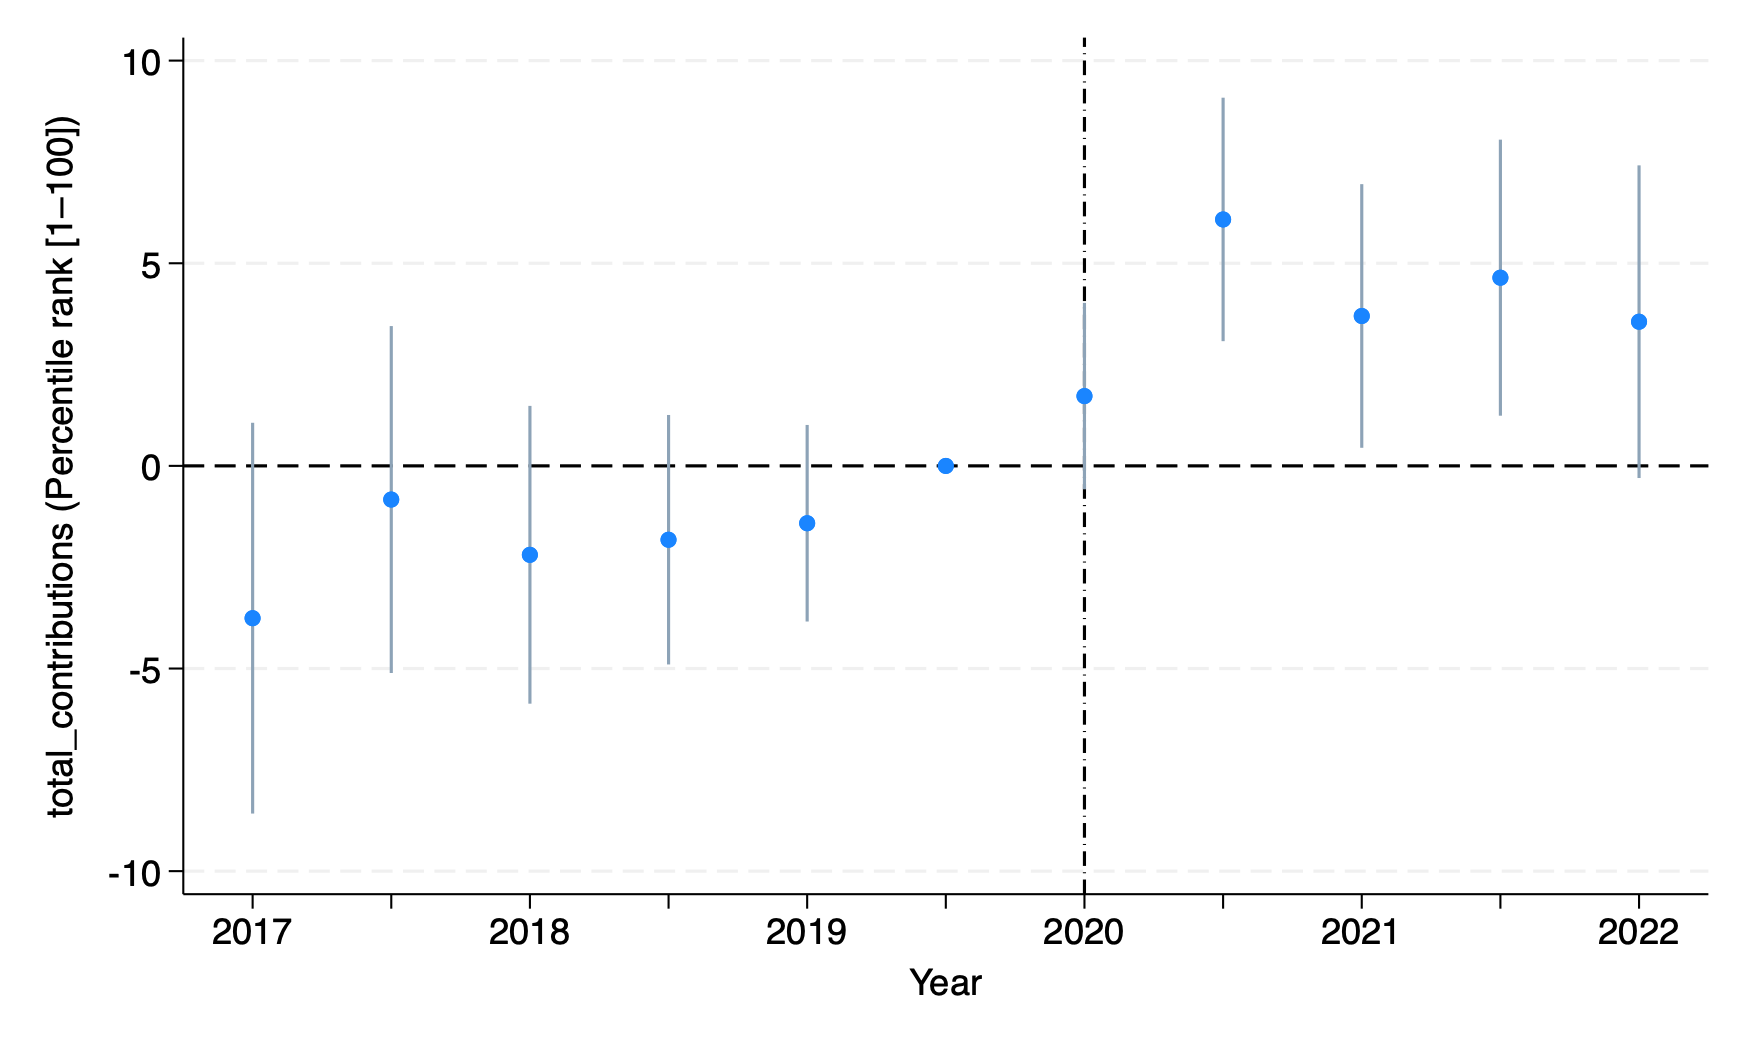
\includegraphics[width=0.9\textwidth]{\cleanedresultsdir/ols_total_contributions_q100.png}\\[2pt]
  \caption*{OLS – Total Contributions}
  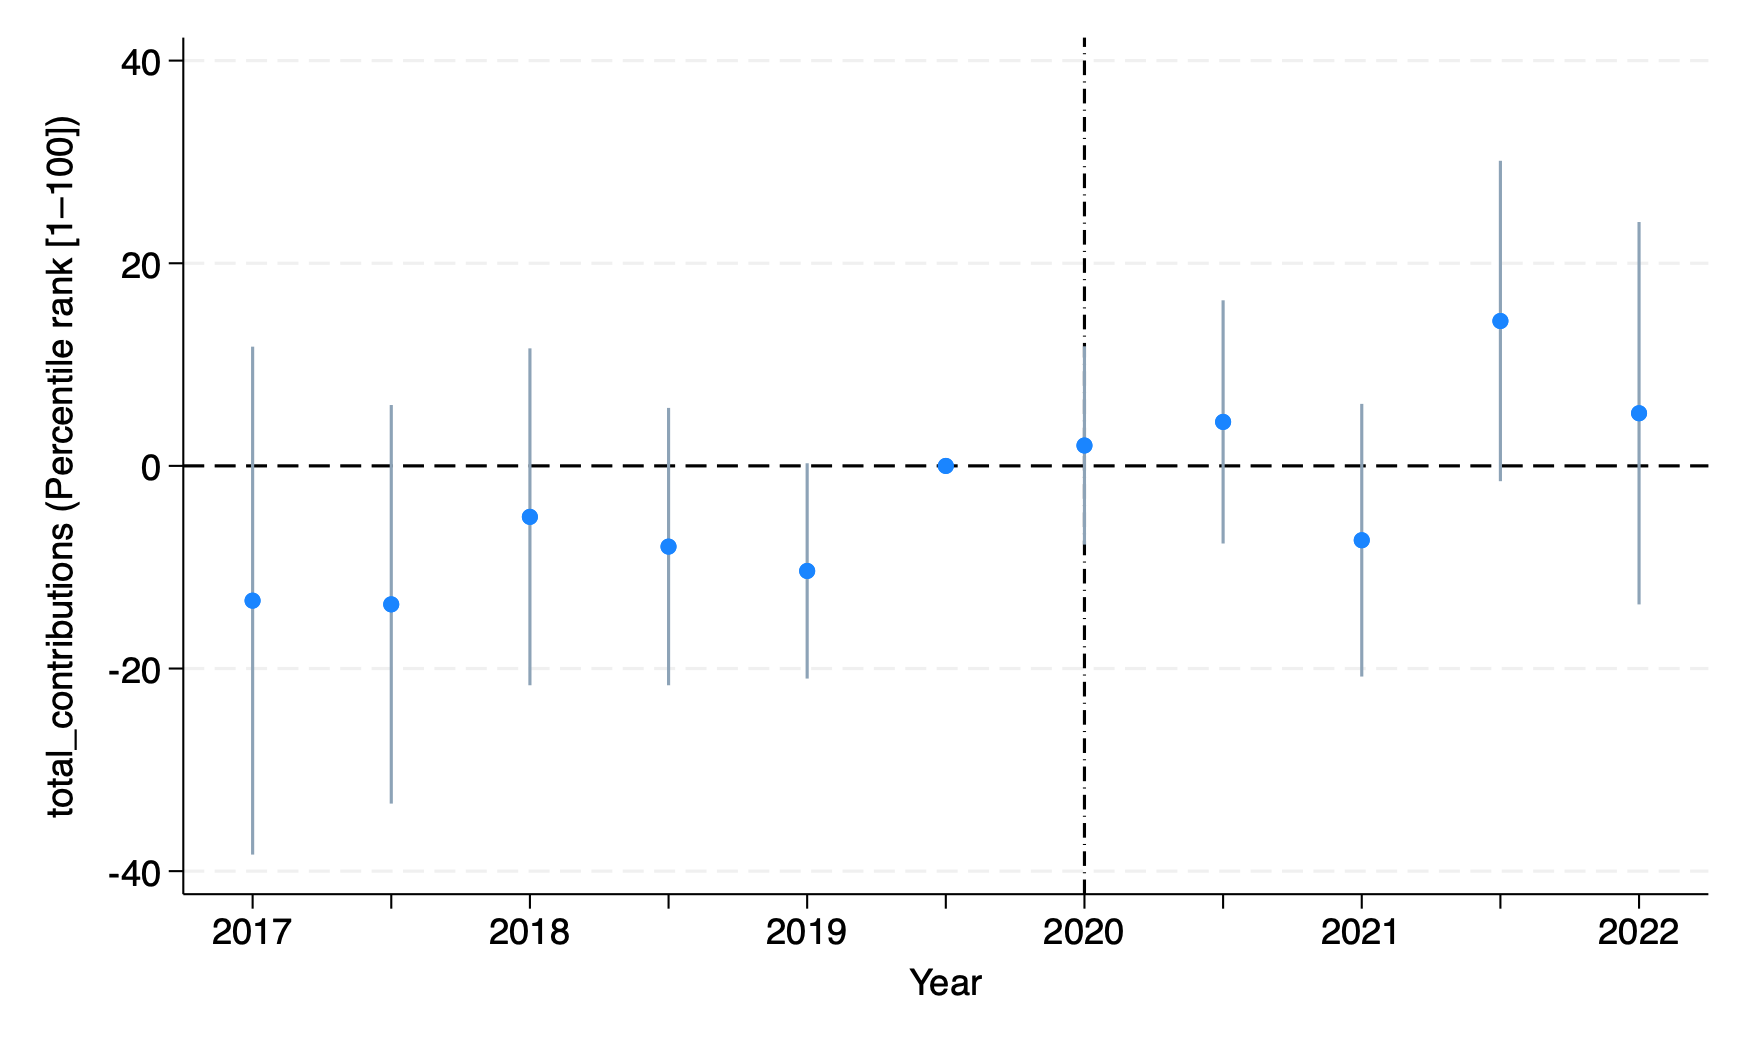
\includegraphics[width=0.9\textwidth]{\cleanedresultsdir/iv_total_contributions_q100.png}\\[2pt]
  \caption*{IV – Total Contributions}
\end{figure}

\clearpage

\begin{figure}[H]
  \centering
  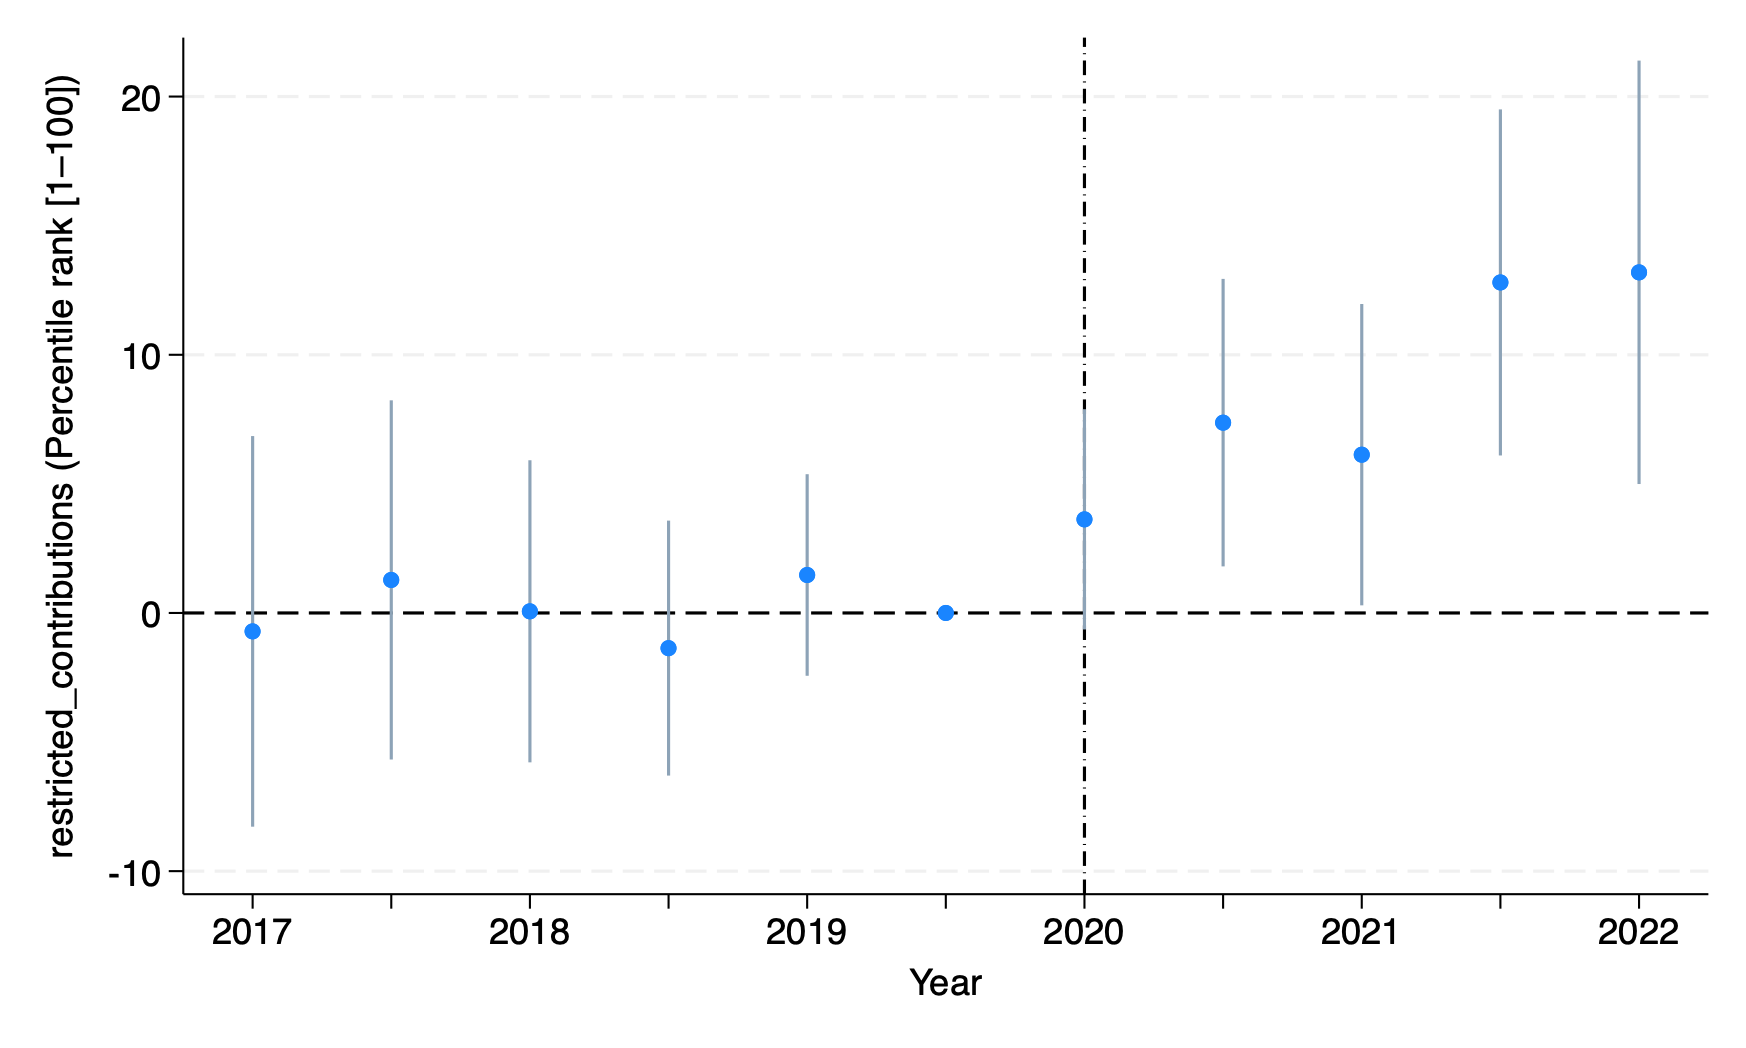
\includegraphics[width=0.9\textwidth]{\cleanedresultsdir/ols_restricted_contributions_q100.png}\\[2pt]
  \caption*{OLS – Restricted Contributions}
  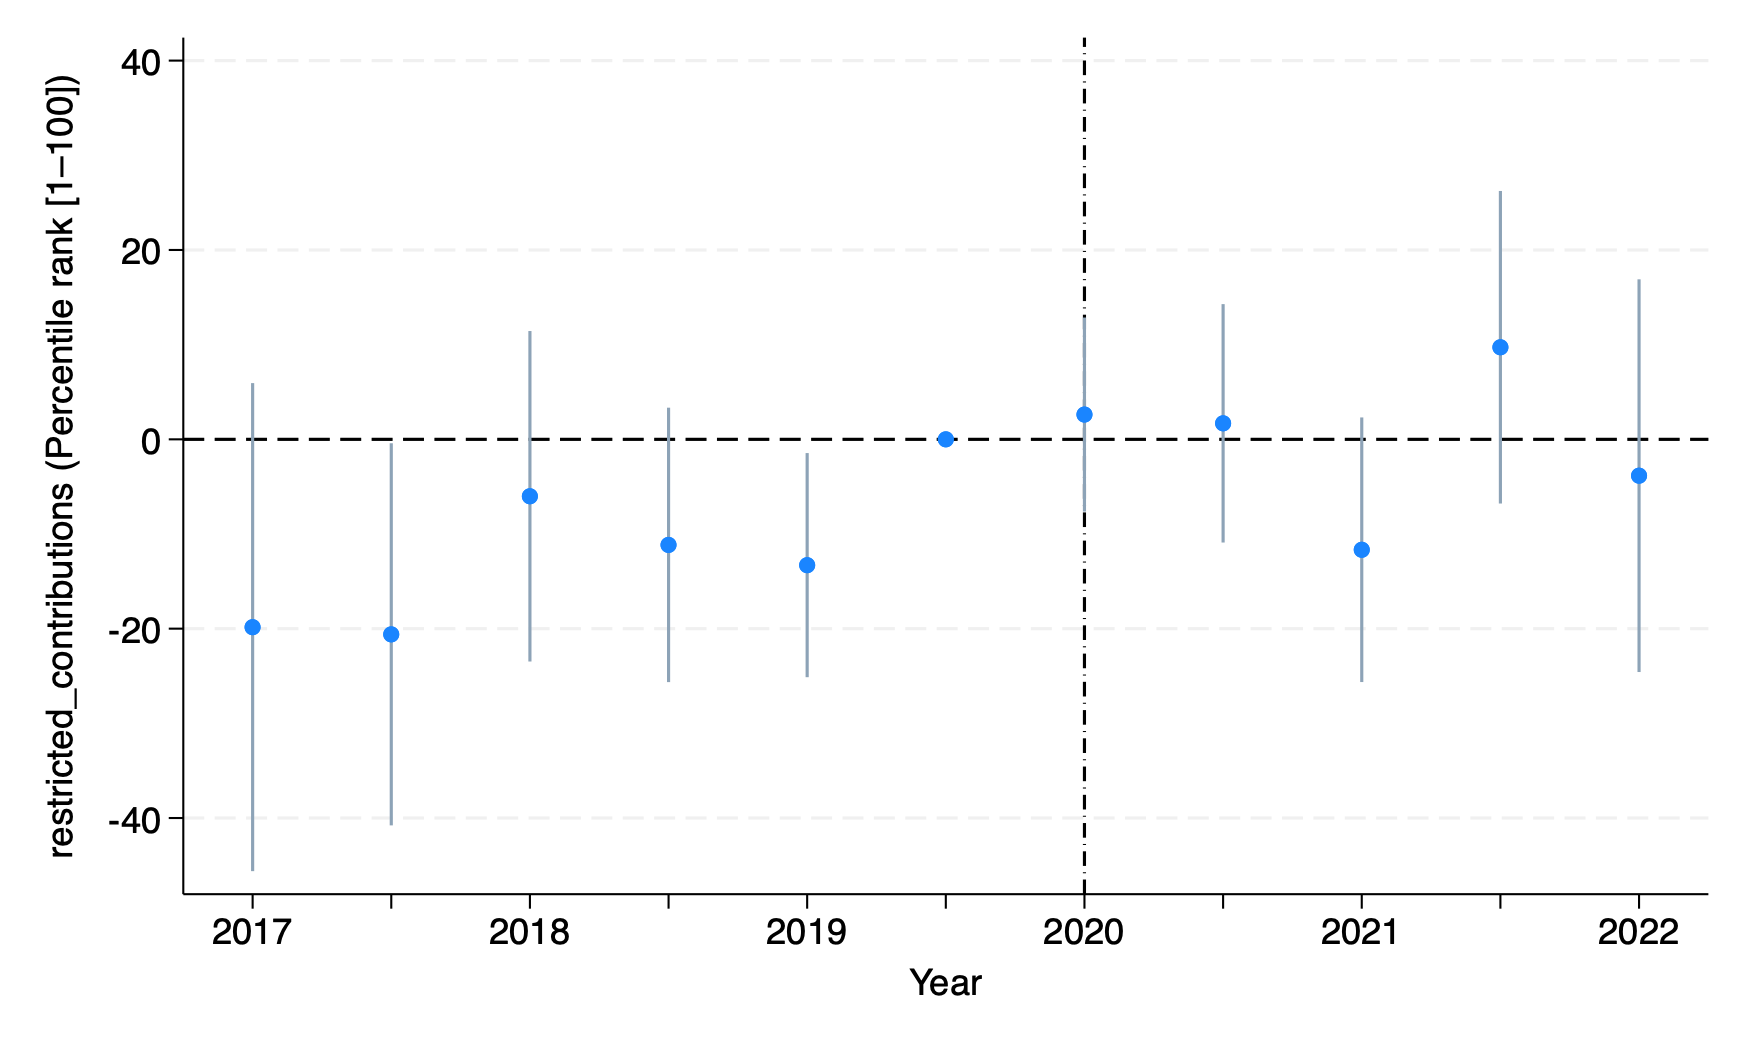
\includegraphics[width=0.9\textwidth]{\cleanedresultsdir/iv_restricted_contributions_q100.png}\\[2pt]
  \caption*{IV – Restricted Contributions}
\end{figure}

\clearpage

% ------------------------------------------------------------------
%  Firm-level outcomes
% ------------------------------------------------------------------

\begin{figure}[H]
  \centering
  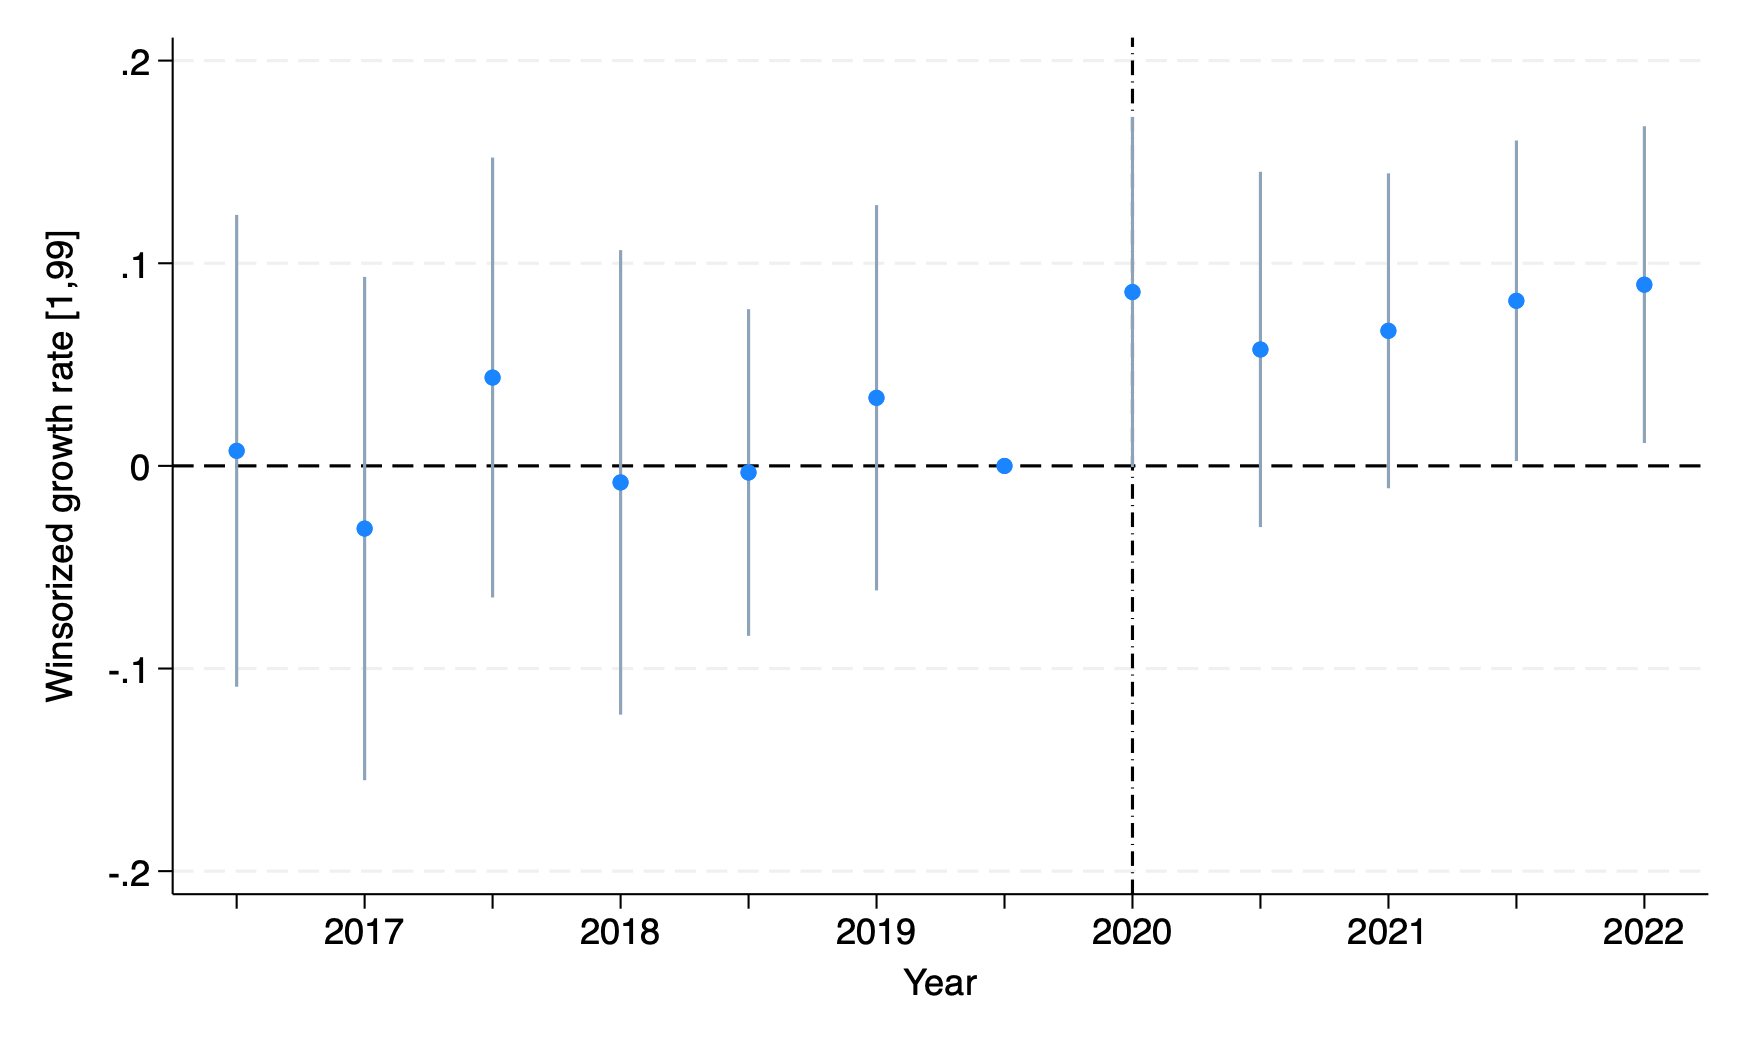
\includegraphics[width=0.9\textwidth]{\cleanedresultsdir/ols_growth_rate_we.png}\\[2pt]
  \caption*{OLS – Employment Growth}
  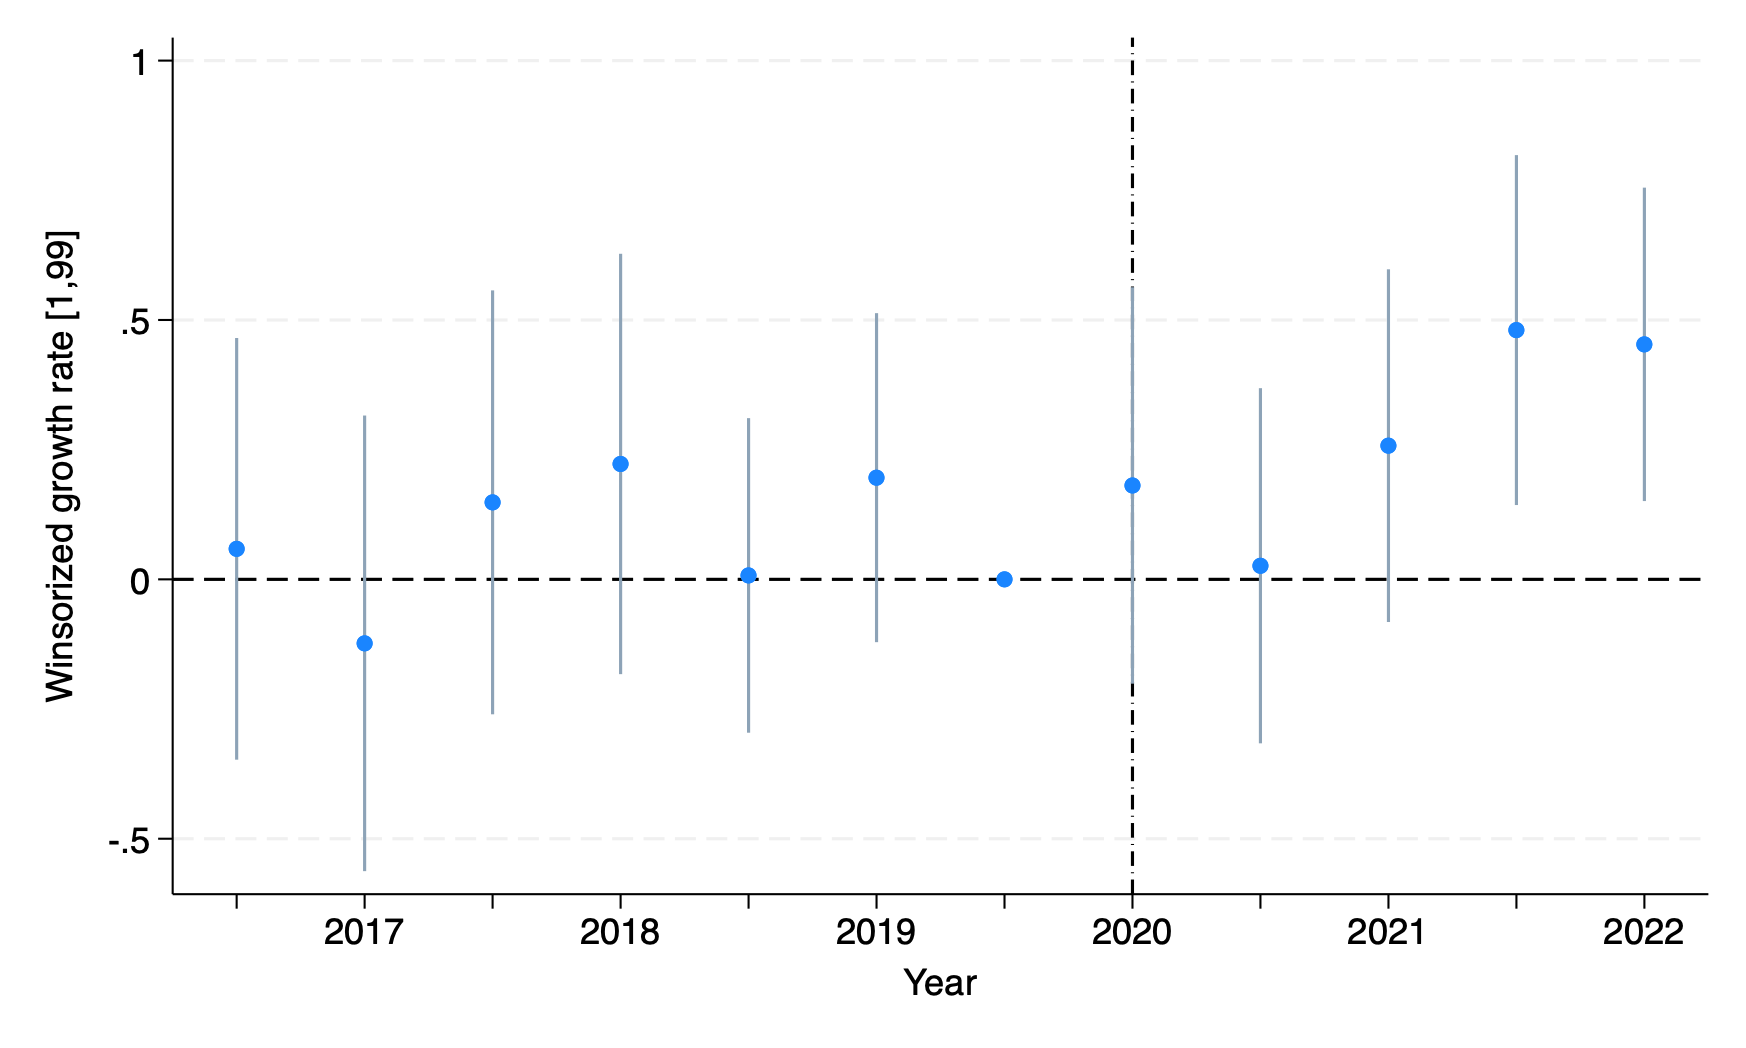
\includegraphics[width=0.9\textwidth]{\cleanedresultsdir/iv_growth_rate_we.png}\\[2pt]
  \caption*{IV – Employment Growth}
\end{figure}

\clearpage

\begin{figure}[H]
  \centering
  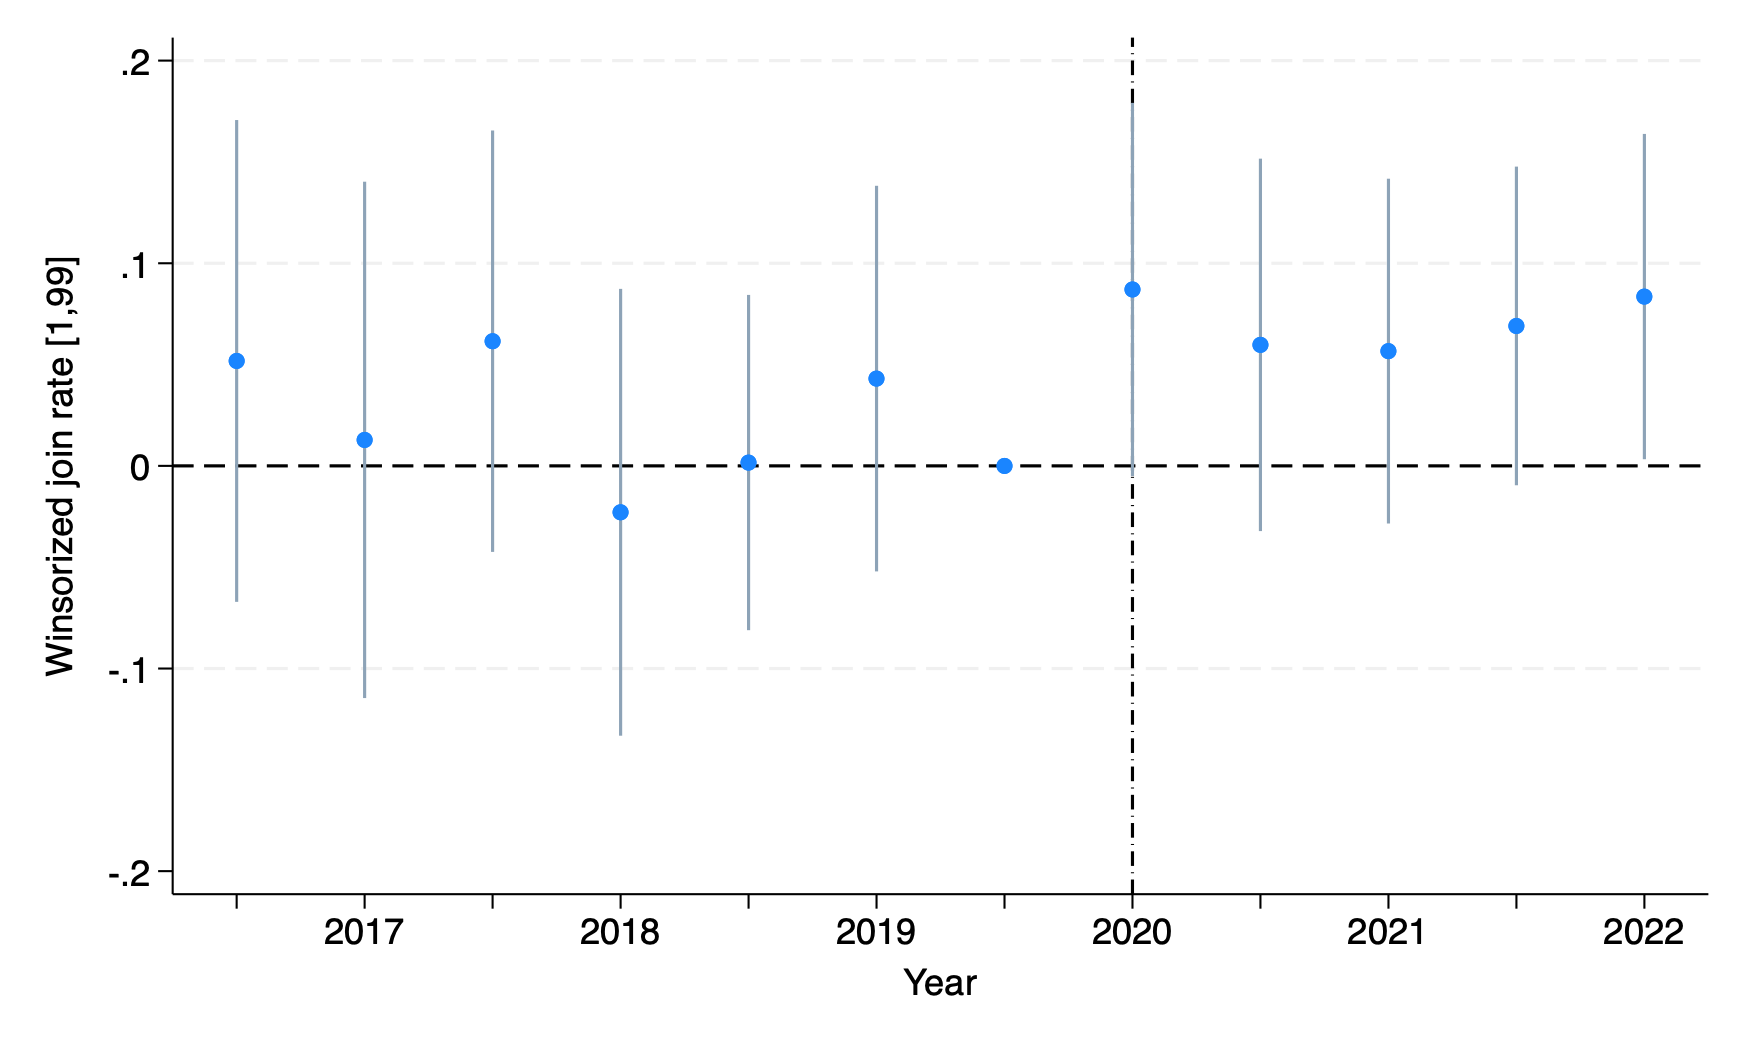
\includegraphics[width=0.9\textwidth]{\cleanedresultsdir/ols_join_rate_we.png}\\[2pt]
  \caption*{OLS – Join Rate}
  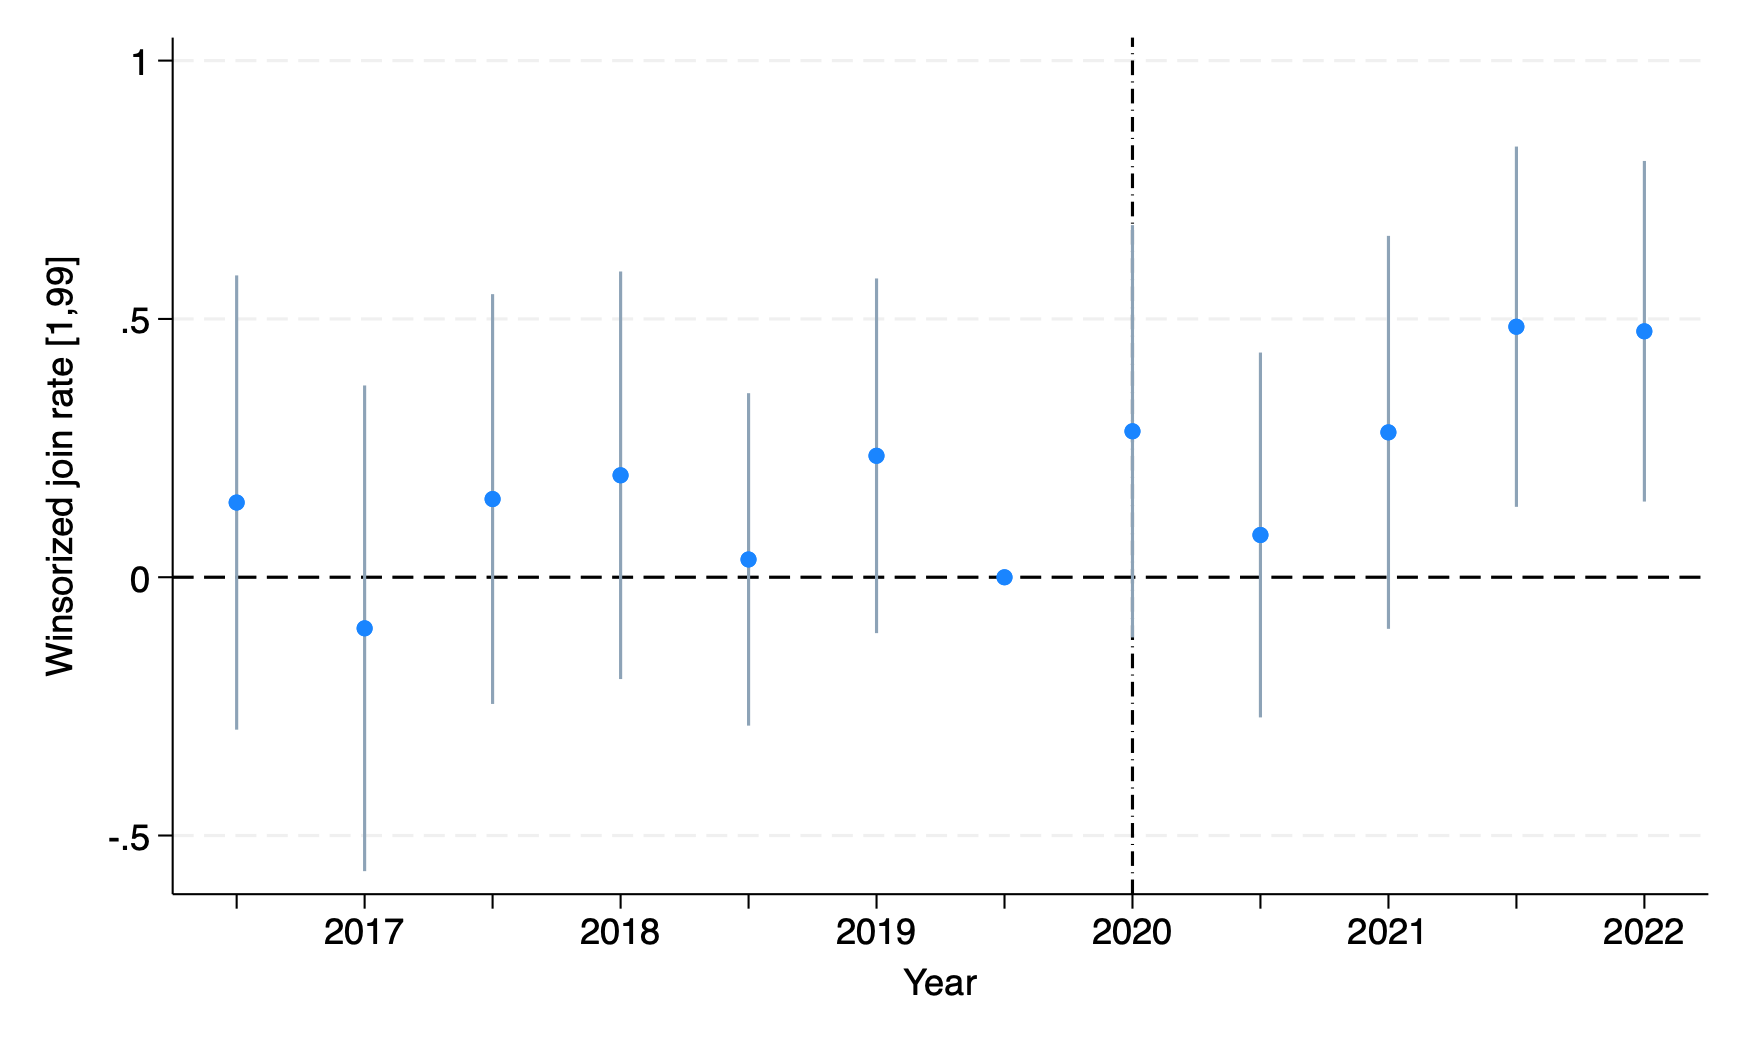
\includegraphics[width=0.9\textwidth]{\cleanedresultsdir/iv_join_rate_we.png}\\[2pt]
  \caption*{IV – Join Rate}
\end{figure}

\clearpage

\begin{figure}[H]
  \centering
  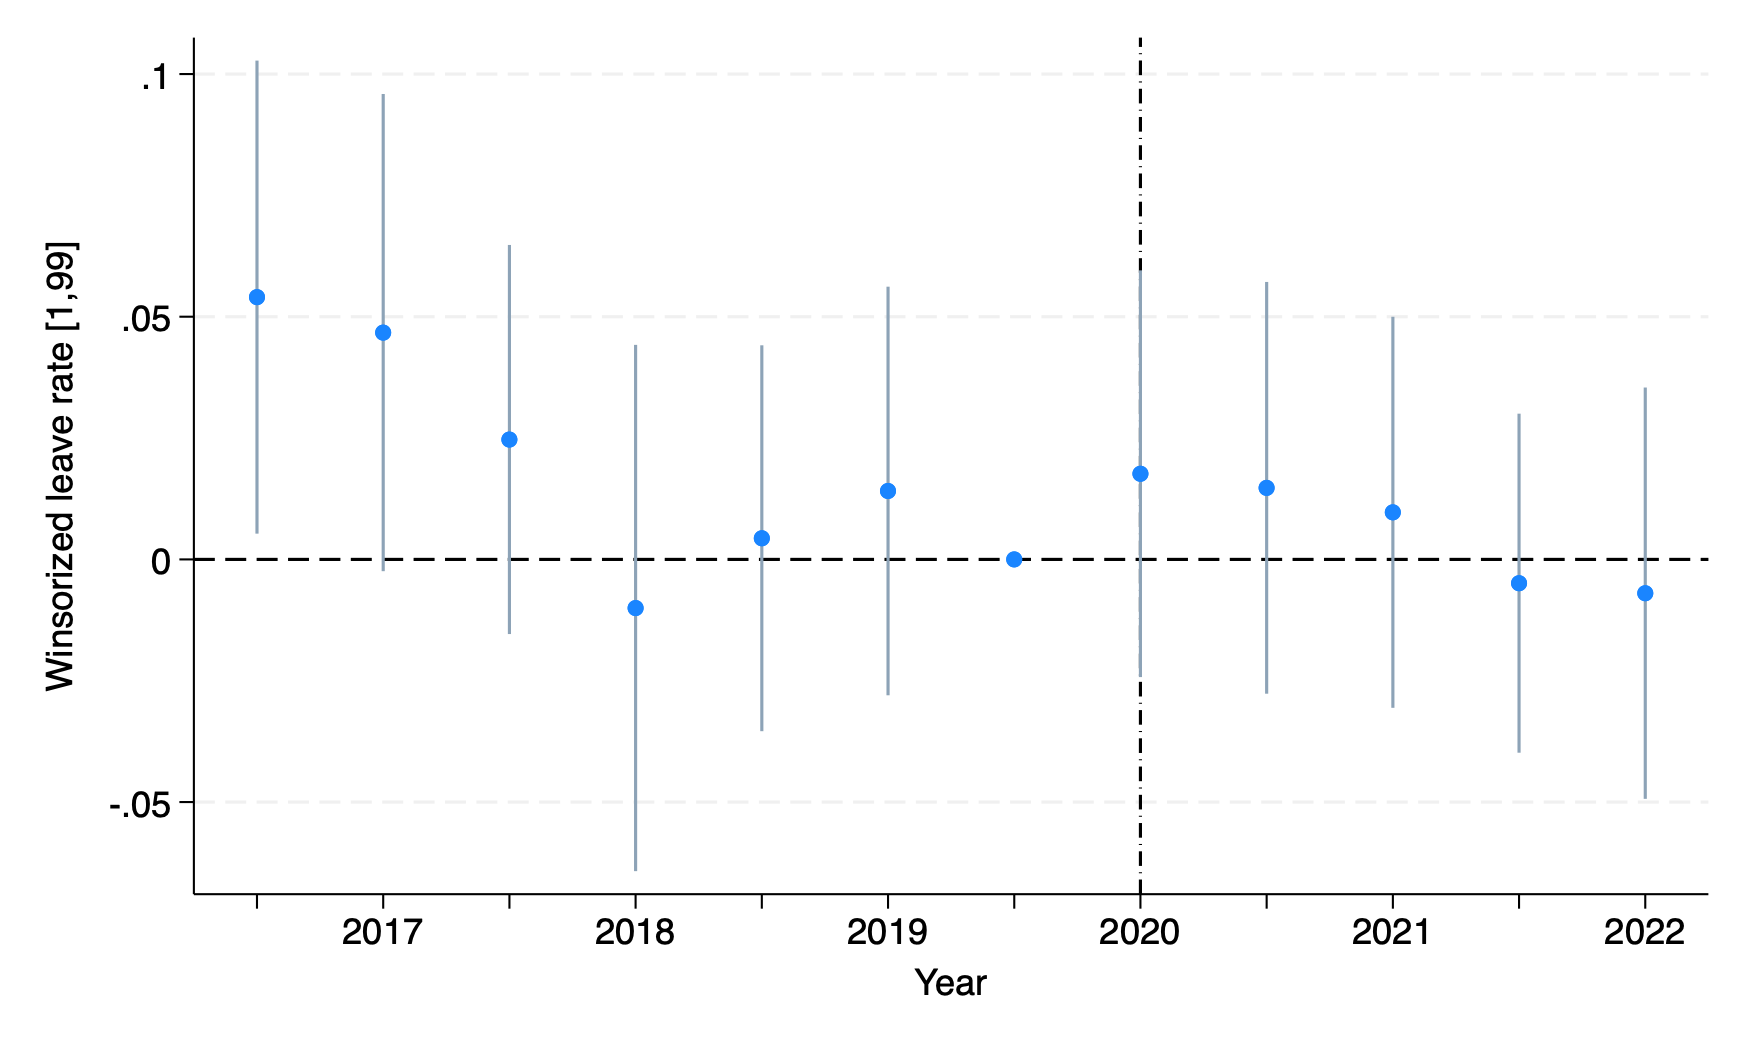
\includegraphics[width=0.9\textwidth]{\cleanedresultsdir/ols_leave_rate_we.png}\\[2pt]
  \caption*{OLS – Leave Rate}
  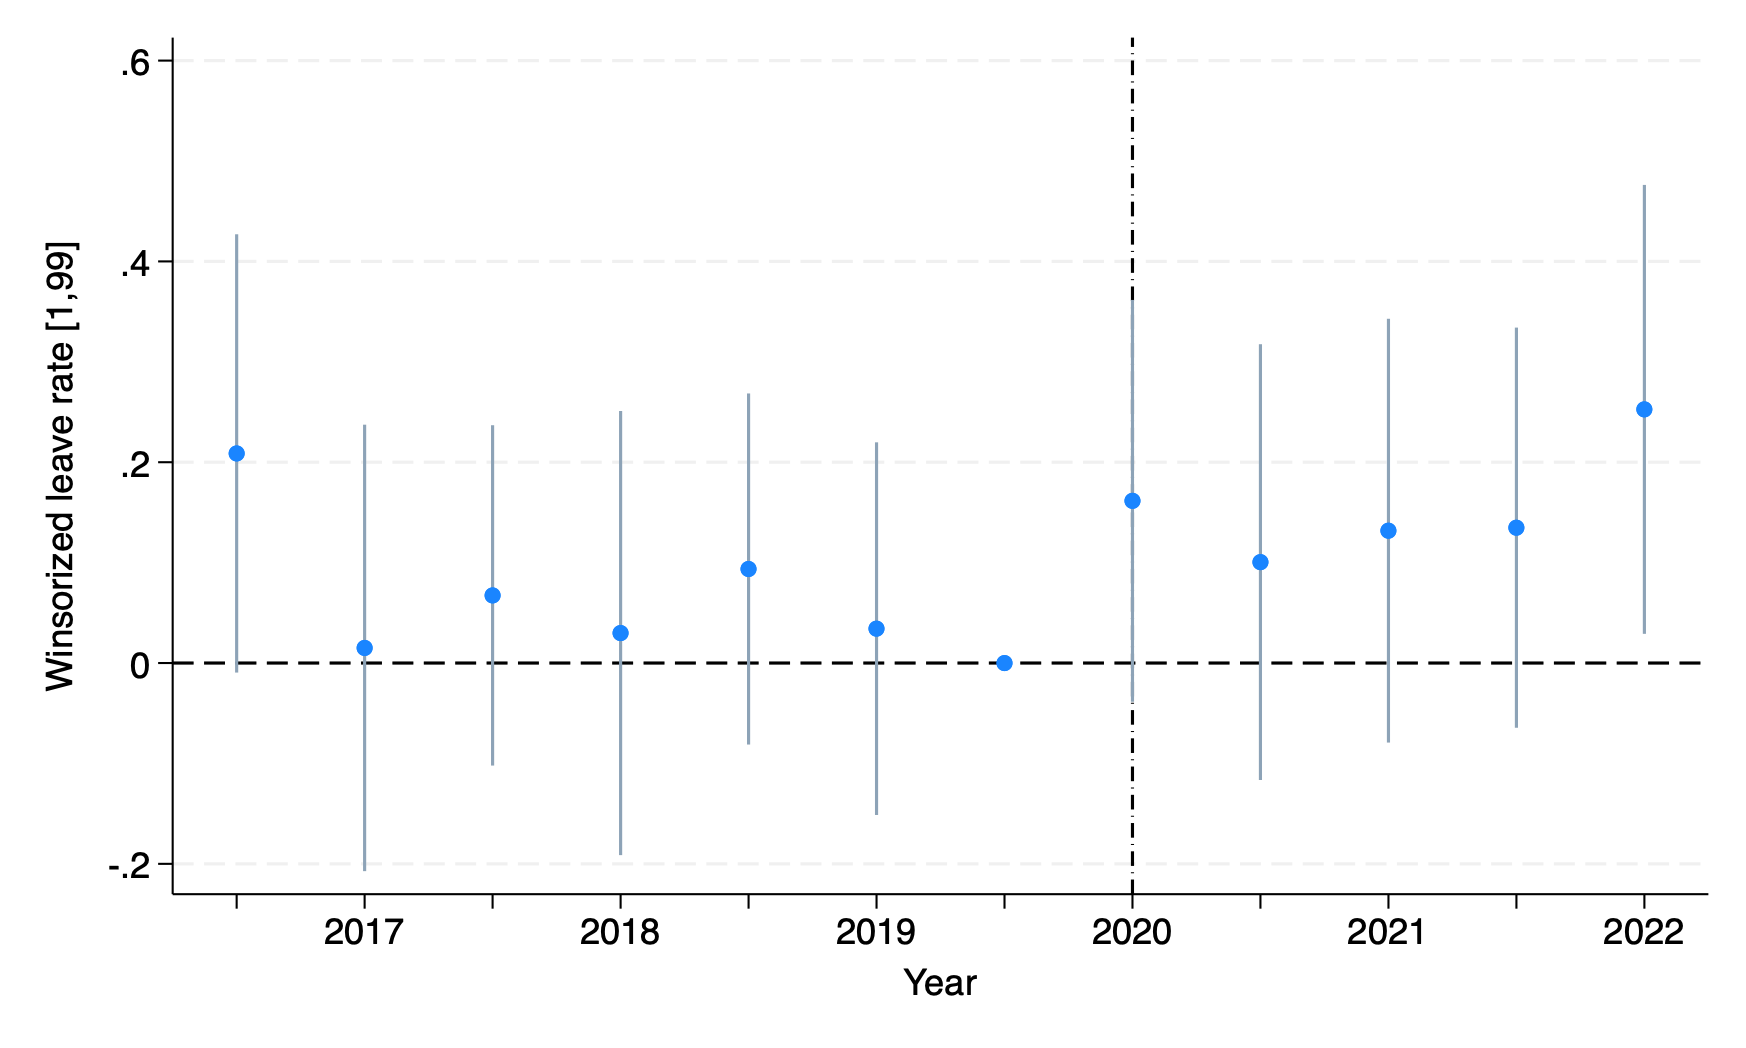
\includegraphics[width=0.9\textwidth]{\cleanedresultsdir/iv_leave_rate_we.png}\\[2pt]
  \caption*{IV – Leave Rate}
\end{figure}


\end{document}
